% Created 2025-05-28 Ср 04:40
% Intended LaTeX compiler: pdflatex
\documentclass[14pt,a4paper,oneside,openany]{extbook}
% Настройка полей (левое: 30 мм, правое: 15 мм (можно 10 мм), верхнее: 20 мм, нижнее: 20 мм)
\usepackage[a4paper,top=20mm,bottom=20mm,left=30mm,right=15mm]{geometry}
% Межстрочный интервал 1.5 (14 пт рекомендуемый размер шрифта, можно задавать через документ или в настройках Overleaf)
\usepackage{setspace}
% \usepackage{mathptmx}
\onehalfspacing
\usepackage{cmap}

% русские буквы
\usepackage[utf8]{inputenc}
\usepackage[T2A]{fontenc}
\usepackage{svg}

\renewcommand{\contentsname}{Содержание}
\usepackage[main=russian,english]{babel}
\newcommand{\MyTOC}{%
  \chapter*{СОДЕРЖАНИЕ}%
  \setcounter{page}{6}
  \markboth{СОДЕРЖАНИЕ}{}%
  \vspace{-3.5cm}%
  {%
    \renewcommand{\contentsname}{}%
    \tableofcontents
  }%
}

% Абзацный отступ 1.25 см
\setlength{\parindent}{1.25cm}
\setlength{\parskip}{0pt}

% Нумерация страниц: арабскими цифрами, по центру нижней части
\usepackage{fancyhdr}
\pagestyle{plain}
\fancyhf{}
\cfoot{\thepage}

% Настройка заголовков через titlesec
\usepackage{titlesec}
% Заголовки глав: прописными буквами, полужирно, по центру, без точки в конце
\titleformat{\chapter}[hang]{\bfseries\Large\centering}{\thechapter}{1em}{}
% Заголовки разделов и подразделов – с абзацным отступом
\titleformat{\section}[hang]{\bfseries\large}{\thesection}{1em}{}
\titleformat{\subsection}[hang]{\bfseries}{\thesubsection}{1em}{}
\titlespacing{\chapter}{0pt}{0pt}{20pt}
\titlespacing{\section}{0pt}{12pt}{6pt}
\titlespacing{\subsection}{0pt}{6pt}{3pt}

% Настройка содержания: точечные лидеры между заголовками и номерами страниц
\usepackage{tocloft}
\renewcommand{\cftdotsep}{1}
\renewcommand{\cftchapleader}{\cftdotfill{\cftdotsep}}

% Подключаем отдельные конфигурационные файлы для списков, формул, таблиц и изображений
% \input{configs/config-lists.tex}
\usepackage{enumitem}
\setlist{nosep} % Убирает дополнительные отступы между элементами списков
\setlist[itemize]{leftmargin=*, label=\textbullet}
\setlist[enumerate]{leftmargin=*}
%%%%%%%%%%%%%%
% \input{configs/config-formulas.tex}
\usepackage{amsmath}
\numberwithin{equation}{chapter} % Формулы нумеруются по главам (например, (1.1), (1.2) и т.д.)
%%%%%%%%%%%%%
% \input{configs/config-tables.tex}
% Подключаем нужные пакеты для таблиц и оформления
\usepackage{booktabs}   % Для красивых горизонтальных линий (\toprule, \midrule, \bottomrule)
\usepackage{multirow}   % Для объединения ячеек по вертикали
\usepackage{float}
\usepackage{caption}    % Для \ContinuedFloat (продолжение таблицы)
\usepackage{longtable}
\usepackage{etoolbox}

\sloppy   % Избавляемся от переполнений
\clubpenalty=10000    % Запрещаем разрыв страницы после первой строки абзаца
\widowpenalty=10000   % Запрещаем разрыв страницы после последней строки абзаца

\usepackage{color}
\usepackage[svgnames]{xcolor}
\usepackage{listings}

\DeclareCaptionLabelSeparator{emdash}{\space---\space}  % пробел, длинное тире, пробел

\captionsetup[table]{position=t, singlelinecheck=false, justification=raggedright, labelsep=emdash, name=Таблица}
\captionsetup[figure]{position=b, singlelinecheck=false, labelsep=emdash, justification=centering, name=Рисунок}
% Настройка выравнивания заголовков

% Переключатель для смены выравнивания заголовков
\newcommand*\RightCaption{\captionsetup{justification=raggedleft}}
\newcommand*\LeftCaption{\captionsetup{justification=raggedright}}
%%%%%%%%%%%%

% Дополнительные пакеты
\usepackage[backend=biber,style=gost-numeric,sorting=none]{biblatex}
\usepackage{booktabs}

\newcommand\YAMLcolonstyle{\color{red}\mdseries}
\newcommand\YAMLkeystyle{\color{black}\bfseries}
\newcommand\YAMLvaluestyle{\color{blue}\mdseries}

\makeatletter

\newcommand\language@yaml{yaml}

\expandafter\expandafter\expandafter\lstdefinelanguage
\expandafter{\language@yaml}
{
  keywords={true,false,null,y,n},
  keywordstyle=\color{darkgray}\bfseries,
  basicstyle=\YAMLkeystyle\small,                                 % assuming a key comes first
  sensitive=false,
  comment=[l]{\#},
  morecomment=[s]{/*}{*/},
  commentstyle=\color{purple}\ttfamily,
  stringstyle=\YAMLvaluestyle\ttfamily,
  moredelim=[l][\color{orange}]{\&},
  moredelim=[l][\color{magenta}]{*},
  moredelim=**[il][\YAMLcolonstyle{:}\YAMLvaluestyle]{:},   % switch to value style at :
  morestring=[b]',
  morestring=[b]",
  literate =    {---}{{\ProcessThreeDashes}}3
                {>}{{\textcolor{red}\textgreater}}1
                {|}{{\textcolor{red}\textbar}}1
                {\ -\ }{{\mdseries\ -\ }}3,
}

% switch to key style at EOL
\lst@AddToHook{EveryLine}{\ifx\lst@language\language@yaml\YAMLkeystyle\fi}
\makeatother

\newcommand\ProcessThreeDashes{\llap{\color{cyan}\mdseries-{-}-}}
%%%%% Listing %%%%
%New colors defined below
\definecolor{codegreen}{rgb}{0,0.6,0}
\definecolor{codegray}{rgb}{0.5,0.5,0.5}
\definecolor{codepurple}{rgb}{0.58,0,0.82}
\definecolor{backcolour}{rgb}{0.95,0.95,0.92}
\definecolor{whitesmoke}{rgb}{0.96, 0.96, 0.96}

\lstdefinestyle{listingstyle}{
  backgroundcolor=\color{backcolour},
  commentstyle=\color{codegreen},
  keywordstyle=\color{magenta},
  numberstyle=\tiny\color{codegray},
  stringstyle=\color{codepurple},
  basicstyle=\ttfamily\footnotesize,
  breakatwhitespace=false,
  breaklines=true,
  captionpos=b,
  keepspaces=true,
  numbers=left,
  numbersep=5pt,
  showspaces=false,
  showstringspaces=false,
  showtabs=false,
  tabsize=4,
  inputencoding=utf8,
  extendedchars=true,
  literate=
    {а}{{\cyra}}1
    {б}{{\cyrb}}1
    {в}{{\cyrv}}1
    {г}{{\cyrg}}1
    {д}{{\cyrd}}1
    {е}{{\cyre}}1
    {ё}{\"{\cyre}}1
    {ж}{{\cyrzh}}1
    {з}{{\cyrz}}1
    {и}{{\cyri}}1
    {й}{{\cyrishrt}}1
    {к}{{\cyrk}}1
    {л}{{\cyrl}}1
    {м}{{\cyrm}}1
    {н}{{\cyrn}}1
    {о}{{\cyro}}1
    {п}{{\cyrp}}1
    {р}{{\cyrr}}1
    {с}{{\cyrs}}1
    {т}{{\cyrt}}1
    {у}{{\cyru}}1
    {ф}{{\cyrf}}1
    {х}{{\cyrh}}1
    {ц}{{\cyrc}}1
    {ч}{{\cyrch}}1
    {ш}{{\cyrsh}}1
    {щ}{{\cyrshch}}1
    {ъ}{{\cyrhrdsn}}1
    {ы}{{\cyrery}}1
    {ь}{{\cyrsftsn}}1
    {э}{{\cyrerev}}1
    {ю}{{\cyryu}}1
    {я}{{\cyrya}}1
    {А}{{\CYRA}}1
    {Б}{{\CYRB}}1
    {В}{{\CYRV}}1
    {Г}{{\CYRG}}1
    {Д}{{\CYR96}}1
    {Е}{{\CYRE}}1
    {Ё}{{\"{\CYRE}}}1
    {Ж}{{\CYRZH}}1
    {З}{{\CYRZ}}1
    {И}{{\CYRI}}1
    {Й}{{\CYRISHRT}}1
    {К}{{\CYRK}}1
    {Л}{{\CYRL}}1
    {М}{{\CYRM}}1
    {Н}{{\CYRN}}1
    {О}{{\CYRO}}1
    {П}{{\CYRP}}1
    {Р}{{\CYRR}}1
    {С}{{\CYRS}}1
    {Т}{{\CYRT}}1
    {У}{{\CYRU}}1
    {Ф}{{\CYRF}}1
    {Х}{{\CYRH}}1
    {Ц}{{\CYRC}}1
    {Ч}{{\CYRCH}}1
    {Ш}{{\CYRSH}}1
    {Щ}{{\CYRSHCH}}1
    {Ъ}{{\CYRHRDSN}}1
    {Ы}{{\CYRERY}}1
    {Ь}{{\CYRSFTSN}}1
    {Э}{{\CYREREV}}1
    {Ю}{{\CYRYU}}1
    {Я}{{\CYRYA}}1
}
\lstset{style=listingstyle} % для красивых листингов
%% Оформление подписей к листингам в стандарте вышки
\DeclareCaptionFormat{modifiedlst}{\lstlistingname~\thelstlisting~--~#3}
\captionsetup[lstlisting]{format=modifiedlst}

% Если язык не поддерживается (например, js) можно добавить свой https://tex.stackexchange.com/questions/89574/language-option-supported-in-listings
% или воспользоваться функцией без выделения синтаксиса через \lstset{style=listingstyle}
\lstdefinestyle{monochromestyle}{
  backgroundcolor=\color{whitesmoke},
  extendedchars=true,
  basicstyle=\footnotesize\ttfamily,
  showstringspaces=false,
  showspaces=false,
  numberstyle=\footnotesize,
  numbersep=9pt,
  breakatwhitespace=false,
  breaklines=true,
  captionpos=b,
  keepspaces=true,
  numbers=left,
  numbersep=5pt,
  showspaces=false,
  showstringspaces=false,
  showtabs=false,
  tabsize=4,
  inputencoding=utf8,
  extendedchars=true,
}

\usepackage[toc]{appendix}
\usepackage{tocloft}
\addto\captionsrussian{%
  \renewcommand{\appendixname}{ПРИЛОЖЕНИЕ}% This is good practice
}

\makeatletter

% Ваша команда \cyrtoc (оставляем как есть)
\def\cyrtoc#1{\ifcase #1\or А\or Б\or В\or Г\or Д\or Е\or Ж\or И\or К\or Л\or М\or Н\or П\or Р\or С\or Т\or У\or Ф\or Х\or Ц\or Ш\or Щ\or Э\or Ю\or Я\else \@ctrerr \fi}

\newcommand\originalappendix{}
\let\originalappendix\appendix

\renewcommand{\appendix}{%
  \label{pg:end} % For referencing the last page number if needed
  \originalappendix % Execute the original \appendix command (from appendix.sty with [toc] option)

  % 1. Redefine chapter numbering for appendices
  \renewcommand{\thechapter}{\cyrtoc{\value{chapter}}}
  % \appendixname is set to "ПРИЛОЖЕНИЕ" for Russian via \addto\captionsrussian in preamble

  % 2. Format chapter titles in the document body using 'titlesec'
}
\makeatother



\usepackage[utf8]{inputenc}
\usepackage[T2A]{fontenc}
\usepackage{graphicx}
\usepackage{longtable}
\usepackage{wrapfig}
\usepackage{rotating}
\usepackage[normalem]{ulem}
\usepackage{amsmath}
\usepackage{amssymb}
\usepackage{capt-of}
\usepackage{hyperref}
\author{Соломатин Роман Игоревич}
\date{}
\title{Разработка фреймфорка по автоматическому определению интентов}
\hypersetup{
 pdfauthor={Соломатин Роман Игоревич},
 pdftitle={Разработка фреймфорка по автоматическому определению интентов},
 pdfkeywords={},
 pdfsubject={},
 pdfcreator={Emacs 30.1 (Org mode 9.7.29)}, 
 pdflang={Russian}}
\usepackage{biblatex}
\addbibresource{~/Desktop/notes/org/bibliography.bib}
\begin{document}

\MyTOC

\chapter*{ТЕРМИНЫ И ОПРЕДЕЛЕНИЯ}
\label{sec:org780e530}
\addcontentsline{toc}{chapter}{ТЕРМИНЫ И ОПРЕДЕЛЕНИЯ}

\emph{AutoML} -- автоматическое машинное обучение.

\emph{NLP} -- обработка естественного языка.

\emph{NLU} -- понимание естественного языка.

\emph{Эмбеддинг} -- это способ числового представления объектов в виде векторов фиксированной размерности

\emph{Промпт} -- это входная инструкция или текстовый запрос, который пользователь (или другая система) передаёт языковой модели.

\emph{Инференс} -- это процесс использования уже обученной модели для получения предсказаний или генерации выходных данных на основе новых входных данных. Во время инференса модель не изменяет своих весов, а лишь применяет выученные зависимости, чтобы выдать ответ или оценку.
\chapter*{Введение}
\label{sec:org3d79ebf}
\addcontentsline{toc}{chapter}{Введение}
В последние годы наблюдается бурный рост интереса к диалоговым системам на основе искусственного интеллекта (чат-ботам, голосовым помощникам и так далее). Так, по данным трендов, интерес к голосовым технологиям AI вырос почти втрое за пять лет\footnote{\url{https://www.verloop.io/blog/100-best-chatbot-statistics}}. Диалоговые системы внедряются в бизнес-процессы и повседневную жизнь, однако создание их интеллектуальной части – модели определения намерения пользователя (intent classification) – остается сложной задачей. Такой модуль является ключевым компонентом системы, позволяя автоматически выявлять цель запроса пользователя, но учет специфики различных доменов серьезно затрудняет разработку универсальной модели. Проектирование и тонкая настройка модели интентов требуют значительных экспертных усилий в области NLP и ML. Поэтому актуальной представляется автоматизация данного процесса – создание универсальных решений, способных уменьшить долю ручной работы и упростить разработку моделей классификации интентов. Автоматизированные подходы к машинному обучению (AutoML) обещают значительно сократить объем ручного труда за счет автоматического подбора оптимальных моделей и параметров, что особенно важно для быстро растущей области диалоговых систем.

На сегодняшний день для задачи классификации интентов накоплен внушительный арсенал методов. Традиционно применяются алгоритмы классического машинного обучения, такие как наивный tf-idf\autocite{joneskarensparck_statistical_1972}, а также подходы на основе k-ближайших соседей и ансамблевые методы (например, градиентный бустинг). С развитием глубокого обучения все более широко используются нейросетевые модели, таких как BERT\autocite{devlin_bert_2019}, которые достигают высоких показателей качества на задачах. Параллельно развиваются технологии AutoML, автоматизирующие выбор моделей и настройку гиперпараметров. Тем не менее, несмотря на прогресс отдельных компонентов, целостных универсальных AutoML-фреймворков, специально ориентированных на определение интентов пользователя, предложено немного. Существующие решения зачастую требуют участия эксперта для каждой новой предметной области, что указывает на необходимость разработать более обобщенный подход.

В связи с этим актуальной является проблема отсутствия универсального, масштабируемого и эффективного AutoML-решения для классификации интентов, способного автоматически адаптироваться к разным доменам без глубокого участия человека-эксперта.

\textbf{Цель исследования} заключается в разработке такого универсального AutoML-фреймворка, который способен автоматически подбирать оптимальные модели и их конфигурации для классификации интентов пользователя. Разработанное решение будет протестировано на различных корпусах данных (наборы пользовательских запросов), а его эффективность сопоставлена с результатами ручной настройки моделей, чтобы оценить выигрыш от автоматизации.

Для достижения поставленной цели в работе решены следующие задачи:
\begin{enumerate}
\item Провести обзор существующих фреймворков и библиотек, применяемых для построения моделей машинного обучения, включая решения для задач классификации пользовательских намерений;
\item Выполнить анализ современных алгоритмов и подходов к задаче определения пользовательских намерений, включая традиционные методы машинного обучения и нейросетевые архитектуры;
\item Разработать концепцию и архитектуру собственного фреймворка создания моделей машинного обучения для классификации пользовательских намерений;
\item Реализовать программную часть фреймворка с возможностью автоматизированной настройки моделей и выбора признаков;
\item Провести экспериментальное исследование эффективности фреймворка на нескольких датасетах из разных предметных областей;
\item Сравнить результаты, полученные с использованием разработанного фреймворка, с качеством моделей, настроенных вручную, и провести анализ полученных результатов.
\end{enumerate}

\textbf{Практическая значимость} работы состоит в том, что созданный AutoML-фреймворк может быть непосредственно применен при разработке реальных диалоговых систем – чат-ботов, голосовых ассистентов, систем клиентской поддержки – и других NLP-приложений. Использование такого инструмента позволит ускорить внедрение новых сервисов и снизить порог вхождения для разработчиков за счет автоматизации подбора оптимальной модели под конкретный набор интентов.

\textbf{Научная новизна} исследования определяется интеграцией современных методов автоматизированного машинного обучения в единой специализированной архитектуре, ориентированной на задачу классификации интентов. В предлагаемом решении объединяются передовые подходы, включая трансформерные модели и методы обучения с малым количеством примеров, в рамках одного AutoML-фреймворка. Такое сочетание технологий нацелено на достижение высокой точности и устойчивости модели при минимальном ручном вмешательстве, что ранее не было реализовано в полной мере для задачи определения интентов пользователя.
\chapter{ОБЗОР ПРЕДМЕТНОЙ ОБЛАСТИ}
\label{sec:orgb4ec570}
\section{Определение намерений пользователя}
\label{sec:org1470ad2}
Классификация намерений –  это задача сопоставления высказывания пользователя с предопределенной меткой намерения (семантической категорией цели пользователя). Например, запрос “Какая погода будет завтра?” может быть классифицирован как запрос погоды. Эта способность является ключевым компонентом понимания естественного языка (NLU) в диалоговых системах, позволяя чат-ботам, виртуальным помощникам и другим агентам искусственного интеллекта понимать, чего хочет пользователь, и соответствующим образом реагировать. Классификация намерений уходит корнями в ранние разговорные диалоговые системы (например, телефонное обслуживание клиентов) и с тех пор получила повсеместное распространение в самых разных областях - от личных помощников и ботов поддержки клиентов до систем медицинских и юридических консультаций.

Ранние методы были основаны на правилах, которые разрабатывались вручную, или на классическом машинном обучении с добавлением дополнительных функций. Однако с развитием области преобладать стали статистические методы, которые основываются на анализе данных. Сначала они использовали традиционные алгоритмы машинного обучения, а затем — методы глубокого обучения. Также мы наблюдаем расширение сферы применения: от простой классификации с закрытым набором параметров, когда каждый запрос должен относиться к одному из известных намерений, до более сложных сценариев. Например, к многоцелевой классификации, обнаружению намерений с открытым доменом или открытым набором параметров (когда запрос не соответствует ни одному из известных намерений), а также к распознаванию намерений с минимальным количеством попыток или вообще без них с помощью мощных генеративных моделей.
Классификация намерений – это задача сопоставления высказывания пользователя с предопределённой меткой, или интентом, отражающим семантическую цель запроса.  Например, запрос “Какая погода будет завтра?” может быть классифицирован как запрос погоды. Эта способность является ключевым компонентом понимания естественного языка (NLU) в диалоговых системах, позволяя чат-ботам, виртуальным помощникам и другим агентам искусственного интеллекта понимать, чего хочет пользователь, и соответствующим образом реагировать. Классификация намерений уходит корнями в ранние разговорные диалоговые системы (например, телефонное обслуживание клиентов) и с тех пор получила повсеместное распространение в самых разных областях - от личных помощников и ботов поддержки клиентов до систем медицинских и юридических консультаций.

Изначально системы классификации намерений строились на вручную заданных правилах и классических алгоритмах машинного обучения с набором признаков. С развитием технологий появились статистические методы и глубокие нейронные сети. Постепенно задачи усложнились – появились мульти-интентная классификация и открытые домены.

Также появилась проблема с запросами, которые не соответствуют ни одному из известных интентов (Out-of-Scope (OOS)) и требуют специальной обработки, чтобы избежать некорректных ответов.

Типичные примеры OOS-запросов: «Какой сейчас курс евро?» в погодном ассистенте, «Как оформить ипотеку?» в кино-ассистенте, «Расскажи, что я ел на прошлой неделе» в системе, не хранящей историю питания. При таких запросах система вежливо отказывается (<<Извините, я не могу помочь с этим запросом<<), предлагает альтернативы или перенаправляет в службу поддержки, а сами OOS-записи сохраняются для расширения набора интентов в будущем.
\section{Методы автоматического машинного обучения}
\label{sec:org4ccd6b0}
Автоматизированное машинное обучение (AutoML) относится к автоматизации полного процесса применения методов машинного обучения для решения реальных задач. Вместо того чтобы вручную выбирать алгоритмы, настраивать гиперпараметры, разрабатывать архитектуры моделей и создавать признаки, система AutoML автоматически принимает эти решения на основе данных. Мотивация для развития AutoML вытекает из бурного роста применения машинного обучения и стремления {}<<демократизировать>>{} машинное обучение – сделать современные техники доступными даже для неспециалистов. Модели машинного обучения зачастую чувствительны к множеству параметров (тип модели, архитектура, настройки гиперпараметров, предварительная обработка признаков и так далее), и нахождение оптимальной конфигурации часто требует кропотливого перебора даже для экспертов. Эта проблема особенно заметна в глубоком обучении, где выбор правильной архитектуры сети и стратегии обучения может определять конечное качество модели. Цель AutoML – автоматизировать принятие этих решений, позволяя пользователю просто предоставить данные, а система подбирает оптимальную модель. Данный обзор литературы предоставляет академический анализ AutoML с основным упором на его применение в обработке естественного языка (NLP), а также включает как фундаментальные работы, так и последние разработки. Мы рассмотрим историческую эволюцию и мотивации AutoML, ключевые технические компоненты, ведущие фреймворки и системы, особенности применения AutoML в задачах NLP (например, классификация текстов, маркировка последовательностей, языковое моделирование), сравнительный анализ производительности и существующие бенчмарки, а также новые тенденции и направления исследований (например, интеграция с фундаментальными моделями, обучение с малым количеством примеров, объяснимость моделей). Обзор ссылается на рецензируемые публикации и академические источники.
\subsection{H2O}
\label{sec:orga2114f9}
H2O\autocite{ledell_h2o_2020} -- является платформой машинного обучения с открытым исходным кодом, разработанной для автоматизации процесса контролируемого обучения. Она ориентирована на выполнение таких задач, как бинарная классификация, многоклассовая классификация и регрессия. Основная функция AutoML в H2O заключается в обучении широкого спектра алгоритмов, включая градиентные повышающие машины, случайные леса, глубокие нейронные сети и обобщенные линейные модели. Затем эти модели объединяются в ансамбль для получения наилучших предсказаний. Результатом работы AutoML является таблица лидеров — ранжированный список моделей по показателям производительности, из которого можно выбрать оптимальную модель для развертывания.

Процесс автоматизации в H2O ограничен по времени, что позволяет пользователю задать максимальное время выполнения или количество моделей. Система обучает столько моделей, сколько возможно в рамках установленных ограничений. В отличие от более сложных методов оптимизации гиперпараметров (например, байесовской оптимизации), H2O использует случайный перебор моделей, полагаясь на разнообразие моделей и ансамблевую технику для достижения высокой производительности. Особенностью платформы является автоматическое создание двух сложенных ансамблей: один включает все обученные модели, другой — только лучшие модели каждого семейства алгоритмов. Этот подход позволяет повысить точность предсказаний без ручной настройки.

H2O эффективно обрабатывает большие массивы данных за счет распределения вычислений по нескольким ядрам или узлам кластера. Платформа реализована на языке Java и предоставляет API для Python, R и других языков, что позволяет интегрировать её в различные среды. Результаты работы легко интерпретируемы: на выходе формируется ранжированный список моделей с указанием показателей производительности и времени обучения. Кроме того, встроенные инструменты объяснения моделей позволяют пользователям получать такие пояснения, как важность переменных, графики частичной зависимости и значения SHAP для лучших моделей. Таким образом, H2O обеспечивает возможность построения множества моделей за короткий промежуток времени, что особенно актуально при работе с большими объемами данных.
\subsection{LightAutoML}
\label{sec:org958513a}
LightAutoML\autocite{vakhrushev_lightautoml_2022} (LAMA) — это облегчённый фреймворк AutoML с открытым исходным кодом, предназначенный для моделирования табличных данных. Основное назначение LAMA — автоматическая генерация конвейеров для структурированных данных с акцентом на скорость и эффективность использования вычислительных ресурсов. Он поддерживает задачи бинарной и многоклассовой классификации, а также регрессию. Изначально ориентированный на работу с табличными данными, LightAutoML расширил свои возможности и теперь поддерживает текстовые признаки.

Фреймворк автоматически выполняет предварительную обработку данных, включая очистку и кодирование отсутствующих значений, вывод типов признаков и их отбор в рамках конвейера. Гиперпараметры моделей настраиваются автоматически. LightAutoML предоставляет готовые пресеты конвейеров (например, {}<<TabularAutoML>>{}), которые обеспечивают быстрое развертывание моделей с минимальным вмешательством пользователя. Также доступны гибкие настройки для создания собственных конвейеров с учетом специфики задачи.

Отличительной чертой LightAutoML является параллельное обучение нескольких конвейеров, результаты которых объединяются с использованием ансамблевых методов. Это может быть простое усреднение или более сложное построение, при котором модели одного уровня используют предсказания предыдущего уровня в качестве входных данных. Также важной концепцией является разделение этапов чтения и предварительной обработки: компонент {}<<Reader>>{} проверяет исходный набор данных и определяет необходимые преобразования для различных типов признаков. Это гарантирует надежность и автоматизацию оценки модели.
\subsection{AutoGluon}
\label{sec:org3aab0d6}
AutoGluon\autocite{erickson_autogluontabular_2020} -- комплексный инструментарий AutoML с открытым исходным кодом, который поддерживает широкий спектр задач машинного обучения, включая прогнозирование табличных данных, компьютерное зрение, обработку естественного языка и прогнозирование временных рядов. Фреймворк предоставляет специализированные API для каждой задачи, например, TabularPredictor и TextPredictor, что упрощает использование в различных областях.

AutoGluon поддерживает обучение различных моделей: от древовидных алгоритмов (LightGBM, XGBoost\autocite{chen_xgboost_2016}, CatBoost\autocite{dorogush_catboost_2018}) до нейронных сетей (например, трансформеров для текста и сверточных сетей для изображений), а также простых моделей, таких как k-ближайших соседей и линейные модели. Пользователь может настроить гиперпараметры, выбрать конкретные модели для обучения и использовать предустановленные конфигурации. Таким образом, AutoGluon предоставляет гибкие возможности для настройки обучения с минимальным объемом кода.
\subsection{FEDOT}
\label{sec:orgc2576d6}
FEDOT\autocites{nikitin_automated_2022}[][]{polonskaia_multiobjective_2021}(Flexible Evolutionary Design of Optimal Trees) -- фреймворк AutoML с акцентом на оптимизацию конвейеров с помощью эволюционных алгоритмов. Разработанный лабораторией моделирования природных систем Университета ИТМО, он предназначен для автоматизации полного жизненного цикла машинного обучения: от предварительной обработки данных до построения и оптимизации моделей.

Основная идея FEDOT -- создание составных конвейеров с помощью генетических алгоритмов. Конвейер представлен в виде направленного ациклического графа (DAG), узлы которого могут быть как преобразованиями данных, так и моделями. Эволюционный оптимизатор, известный как {}<<GOLEM>>{}, генерирует начальную популяцию случайных конвейеров и затем улучшает их с помощью мутаций и скрещивания. В результате создаются оптимальные конвейеры, адаптированные к конкретной задаче.

FEDOT поддерживает работу с различными типами данных (табличные, текстовые, графовые) и обеспечивает гибкость настройки. Инструменты анализа позволяют исследовать чувствительность компонентов конвейера, а также оценивать влияние отдельных моделей на итоговую производительность. Фреймворк поддерживает экспорт оптимальных конвейеров в формате JSON и позволяет интеграцию в производственные среды.
\subsection{Сравнение алгоритмов}
\label{sec:org1fa8d1a}
Классификация намерений пользователя представляет собой важную задачу в области обработки естественного языка, требующую использования современных методов машинного обучения и автоматизированных инструментов для построения эффективных моделей. Для реализации данной задачи важно учитывать несколько ключевых критериев: способы обработки текста, поддержка работы с малым набором данных, поддержка выявления намерений вне области определения (Out-Of-Scope, OOS), гибкость настройки параметров, поддержка логирования и возможность использования промптов для энкодеров.

Первым важным критерием является обработка текста, поскольку текстовые данные являются основным источником информации при классификации намерений. Современные модели, такие как трансформеры, демонстрируют высокую точность в задачах NLP благодаря обучению на больших объемах текстов. Поэтому наличие встроенной поддержки текстовых признаков, включая возможность применения эмбеддингов и трансформерных архитектур, является важным аспектом при создании фреймворка.

Вторым значимым критерием является поддержка работы с малым набором данных. В прикладных задачах, связанных с классификацией намерений, часто возникает ситуация, когда количество размеченных данных ограничено. Это особенно актуально при адаптации моделей к новым доменам или редким языковым конструкциям. Поэтому важной характеристикой фреймворка является его способность эффективно работать с малыми наборами данных, например, за счет использования регуляризации или предварительно обученных эмбеддингов.

Не менее важной является поддержка Out-Of-Scope (OOS) -- задачи, заключающейся в выявлении запросов пользователя, выходящих за рамки известных классов намерений. Выявление OOS-классов критично для обеспечения надежности и безопасности систем, поскольку позволяет корректно обрабатывать неизвестные или неподдерживаемые запросы. Фреймворки, реализующие данную функциональность, позволяют обучать модели, способные распознавать не только заданные классы, но и детектировать аномальные данные.

Следующим важным аспектом является изменение параметров запуска. В зависимости от задачи, объема данных и доступных вычислительных ресурсов, может потребоваться гибкая настройка процесса обучения. Это особенно актуально при разработке моделей для различных доменов или на основе разнородных данных. Возможность адаптировать параметры позволяет оптимизировать модель как по точности, так и по времени выполнения.

Поддержка логирования является важным компонентом автоматизации машинного обучения, поскольку позволяет отслеживать процесс обучения, хранить промежуточные результаты и проводить анализ моделей. В контексте классификации намерений важно иметь возможность анализировать ошибки и проверять гипотезы о моделях на каждом этапе обучения. Логирование помогает выявлять причины ухудшения качества моделей и отслеживать процессы настройки гиперпараметров, что критично для обеспечения повторяемости экспериментов и объяснимости конечных результатов.

Последним критерием является поддержка промптов для энкодеров, что особенно важно при использовании моделей на основе трансформеров. В последнее появляются модели, которые поддерживают промпты в зависимости от задачи, которые улучшают качество ее работы. Например, модель e5\autocite{wang_multilingual_2024} использует \texttt{query:} и \texttt{passage:} для создания разных частей эмбеддинга для поиска похожих текста.

Таблица сравнения фреймворков по заданным критериям \ref{tbl:automl_comparison}.

\begin{table}[h!]
\caption{\label{tbl:automl_comparison}Сравнение AutoML фреймворков}
\centering
\begin{tabular}{|p{3cm}|p{3cm}|p{3cm}|p{3cm}|p{3cm}|}
\hline
Критерий & H2O & LightAutoML & AutoGluon & FEDOT\\
\hline
Способы обработки текста & Нет поддежки из коробки & TF-iDF\autocite{joneskarensparck_statistical_1972} и эмбеддинг & Эмбеддинг & TF-iDF, эмбеддинг\\
\hline
Поддержка работы с малым набором данных & Не оптимизирован для малых данных & Имеет режимы, позволяющие работать с небольшими наборами данных & Нет поддержки & Может адаптироваться к малым данным\\
\hline
Изменение параметров запуска & Гибкая настройка через API & Настройка через пресеты и конфигурацию, плохо документировано & Можно передавать свой конфиг, плохо документировано & Ограненная настройка\\
\hline
Поддержка логирования во внешние системы & Логирование результатов через интеграцию с H2O Flow & Нет поддержки & Нет поддержки & Нет поддержки\\
\hline
Поддержка промптов для энкодеров & Нет поддержки & Нет поддержки & Нет поддержки & Нет поддежки\\
\hline
Поддержка OOS (out of scope) & Нет встроенной поддержки & Нет встроенной поддержки & Нет поддержки & Нет поддержки\\
\hline
\end{tabular}
\end{table}
\section{Нейросетевые методы представления текста}
\label{sec:orgb88ee63}
\subsection{BERT}
\label{sec:org2a97a64}
BERT\autocite{devlin_bert_2019} (Bidirectional Encoder Representations from Transformers) — это языковая модель на основе архитектуры трансформера\autocite{vaswani_attention_2017}, которая предобучается на задаче маскированного языкового моделирования и предсказания следующего предложения. В отличие от односторонних моделей вроде GPT\autocite{radford_language_2019} или неглубоких двунаправленных конкатенаций, таких как ELMo\autocite{peters_deep_2018}, BERT одновременно учитывает и левый, и правый контекст на всех слоях, что обеспечивает более глубокое понимание языка.

В своей базовой конфигурации модель содержит 12 «базовых блоков» (слоёв) трансформера, а размер скрытых представлений в каждом из них равен 768. Входной текст разбивается на токены с помощью WordPiece (словарь из 30 000 токенов), затем в начало последовательности добавляется специальный маркер \texttt{[CLS]}, а при подаче пары предложений между ними вставляется \texttt{[SEP]}. К каждому токену добавляются позиционные эмбеддинги и эмбеддинги сегментов, указывающие, к какому из предложений он относится. Представление токена \texttt{[CLS]} служит свёрнутым вектором для задач классификации, а остальные эмбеддинги используются для задачи span‐prediction.

Во время предобучения первая задача — маскирование токенов. 15 \% токенов в каждом примере случайно выбирается для маскировки: 80 \% из них заменяются на \texttt{[MASK]}, 10 \% — на случайный токен, и 10 \% остаются без изменений. Модель пытается угадать исходные токены, опираясь на полный контекст. Такая схема способствует более устойчивому обучению по сравнению с традиционными слева-направо или справа-налево моделями.

Вторая задача — предсказание следующего предложения: с вероятностью 50 \% подаётся пара из действительно идущих друг за другом предложений, а с вероятностью 50 \% — два случайных предложения из корпуса. Модель обучается определять, являются ли они смежными, что развивает понимание связности и логики текста (см. рис. \ref{fig:bert_pretrainin}).

Для решения downstream‐задач BERT требует лишь добавления небольшой выходной головы: для классификации на токен \texttt{[CLS]}, для span‐prediction — двух векторов начала и конца и т. д. Затем все параметры модели дообучаются одновременно, что делает адаптацию универсальной и простой. Абляционные эксперименты показывают, что и двунаправленность внимания, и задача предсказания следующего предложения критически важны: при их исключении эффективность существенно падает, а увеличение глубины и ширины модели даёт стабильный прирост в переносимости представлений.

\begin{figure}[h]
\centering
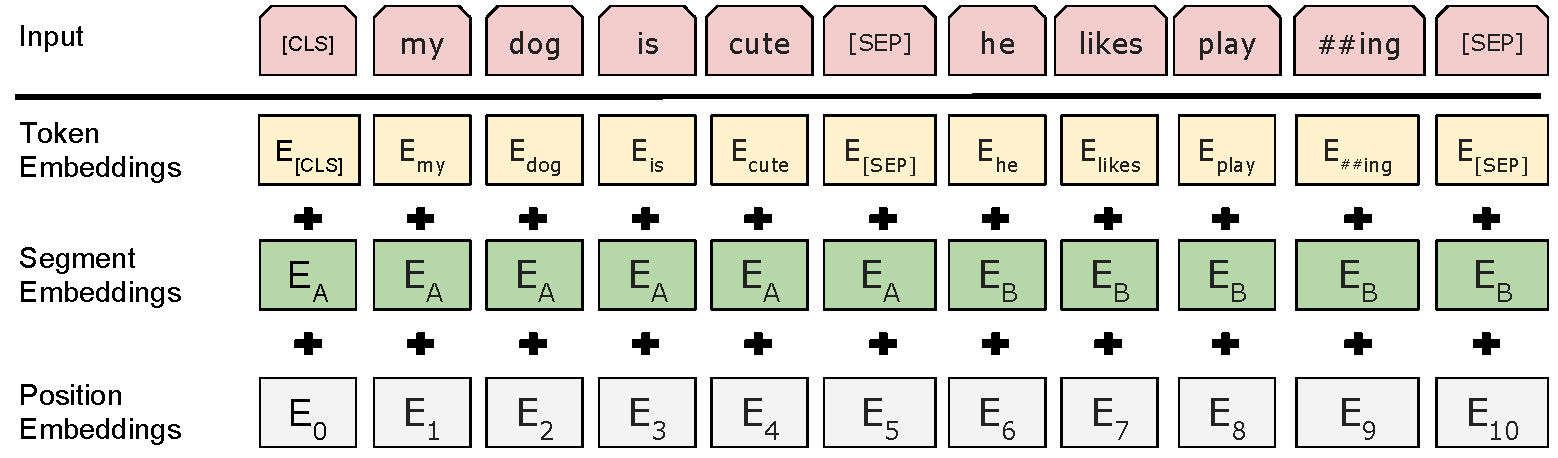
\includegraphics[width=.9\linewidth]{img/Input_Emebeddings.pdf}
\caption{\label{fig:inputemebeddings}Пример преобразования входного текста в эмбеддинги}
\end{figure}

\begin{figure}[h]
\centering
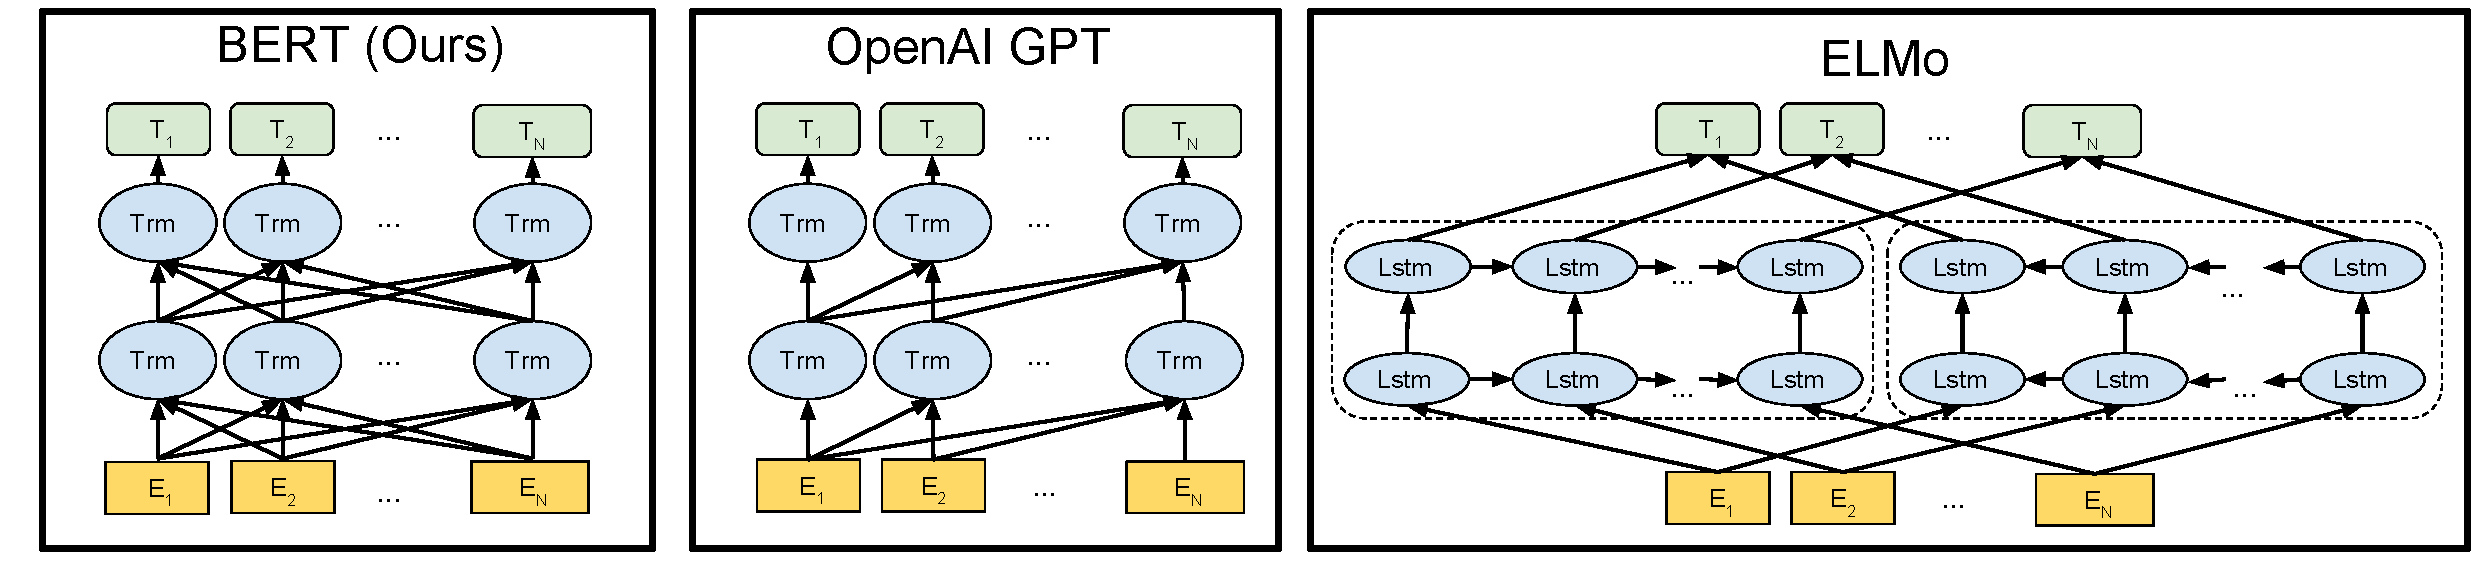
\includegraphics[width=.9\linewidth]{img/BERT_comparisons.pdf}
\caption{\label{fig:BERT_comparisons}Сравнение направленностей внимания ELMo, GPT и BERT}
\end{figure}

\begin{figure}[h]
\centering
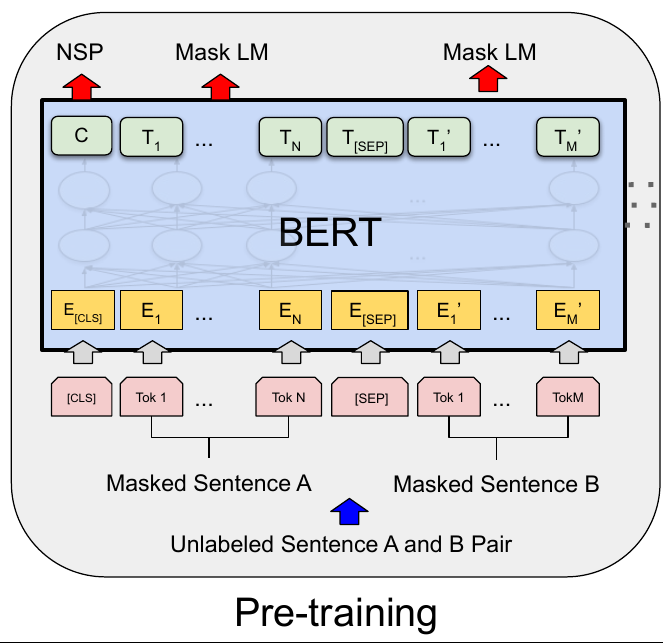
\includegraphics[width=.6\textwidth]{img/bert_pretrainin.png}
\caption{\label{fig:bert_pretrainin}Схема задачи предсказания следующего предложения в BERT}
\end{figure}
\subsection{Sentence Transformers}
\label{sec:org6c8b22c}
Sentence BERT\autocite{reimers_sentencebert_2019} (SBERT) -- модификаця исходной моделей BERT, нацеленная на эффективное построение векторных представлений предложений. В данной работе BERT выступает в роли общего кодировщика, параметры которого разделяются между двумя (или тремя, в случае триплетной версии) ветвями сети, обрабатывающими по отдельности входные предложения. Такое «сиамское» строение (biencoder) позволяет получать фиксированные векторы предложений, сохраняющие богатую семантическую информацию, без необходимости совместной обработки пар предложений на этапе инференса.

Основной этап обучения SBERT заключается в тонкой подгонке предобученного трансформера на разметках задач распознавания естественного вывода (SNLI, Multi-Genre NLI) или семантического сходства (STS). После прохождения каждого предложения через общий энкодер применяются операции агрегирования (mean-, CLS- или max-пулинг), формирующие итоговый эмбеддинг. Для оптимизации используются три различных критерия: классификационный (с дополнительным полносвязным слоем и softmax), регрессионный (минимизация MSE на косинусном сходстве) и триплетная функция потерь (гарантирующая, что «анкоры» ближе к «позитивам», чем к «негативам» на заданный порог).

В результате декомпозиции процедуры сравнения пар предложений и предварительного вычисления эмбеддингов SBERT демонстрирует существенное ускорение: поиск ближайших соседей в корпусе из 10 000 предложений, требовавший ранее десятков часов работы перекрёстного энкодера BERT на GPU, сводится к нескольким секундам при использовании SBERT и быстрых алгоритмов косинусного поиска. Это позволяет применять семантический поиск, кластеризацию и извлечение информации в режиме реального времени и на больших масштабах.

Стоит различать две парадигмы работы с парными входами в трансформерах. Cross-encoder принимает на вход конкатенацию двух предложений, обрабатывает их совместно и выдает прямую оценку сходства (или класс) через полносвязный классификатор — такая схема обеспечивает высочайшую точность, но накладывает квадратичную по размеру корпуса сложность инференса. Biencoder (сиамская или двухветвная модель) кодирует каждое предложение независимо в единое пространство эмбеддингов, после чего сходство вычисляется быстро «на лету» с помощью косинусной меры; это даёт компромисс между качеством и производительностью и лежит в основе SBERT.
\section{Методы адаптации моделей}
\label{sec:orgf7a01cf}
\subsection{P-Tuning}
\label{sec:org36a6e56}
P-Tuning\autocite{liu_gpt_2023} дополняет дискретные подсказки обучаемыми непрерывными эмбеддингами, превращая их в гибридную схему, где модель может автоматически адаптировать ввод под специфику задачи. Вместо жёстко заданных шаблонов к входному тексту добавляется последовательность параметризованных векторов подсказок, которые проходят через облегчённый энкодер (LSTM, MLP или identity) и оптимизируются вместе с моделью или независимо от неё.

Метод решает проблему высокой нестабильности ручных дискретных подсказок, когда даже незначительные изменения формулировки приводят к резкому падению качества. Благодаря обучаемым эмбеддингам P-Tuning снижает разброс результатов при различных вариантах подсказок и позволяет получать более предсказуемый отклик модели.

P-Tuning демонстрирует значительный рост точности и устойчивости на широком спектре задач: от фактического знания (LAMA) до комплексных NLU-бенчмарков (SuperGLUE) и сценариев с ограниченным числом примеров. Этот подход обеспечивает более быструю и надёжную адаптацию моделей к новым задачам без затрат на полный перебор шаблонов.
\subsection{LoRA}
\label{sec:org7a438c5}
LoRA\autocite{hu_lora_2021} (Low-Rank Adaptation) -- метод обучения модели, который замораживает (не обучает) веса предобученной модели и обучает только небольшие низкоранговые матрицы обновлений, что позволяет существенно сократить количество обучаемых параметров и требования к хранению при сохранении полной скорости инференса.

LoRA решает проблему высокой стоимости тонкой настройки всё более крупных моделей на основе трансформеров, при которой обновление всех параметров требует огромных ресурсов GPU. Вместо изменения исходной матрицы весов \(W_0\), LoRA представляет адаптацию \(\Delta W\) как произведение двух значительно меньших матриц, используя тот факт, что эффективные обновления лежат в низкоразмерном подпространстве.

Конкретно, для полносвязанного слоя с \(W_0 \in \mathbb{R}^{d \times k},\) LoRA вводит матрицу \(\Delta W = B\,A,\) где \(A \in \mathbb{R}^{r \times k},\quad B \in \mathbb{R}^{d \times r},\quad r \ll \min(d,k)\). Обучаются только \(A\) и \(B\) (инициализируемые так: \(A \sim \mathcal{N}(0,\sigma^2)\), \(B = 0\)), в то время как \(W_0\) остаётся неизменным. Скалярный множитель \(\tfrac{\alpha}{r}\) масштабирует обновление для стабилизации обучения. Во время работы матрица считается как \(h = W_0\,x + (B\,A)\,x\).

LoRA совместим с другими методами повышения эффективности: в отличие от адаптеров, добавляющих новые слои, или prompt-tuning, расширяющего входную последовательность, он не увеличивает вычислительную сложность и не снижает максимальную длину обрабатываемых последовательностей.
\section{Методы классификации текста}
\label{sec:orga5e87e8}
\subsection{Logistic Regression}
\label{sec:org12299da}
Логистическая регрессия — это статистический метод, используемый для моделирования вероятности двоичного исхода (например, успех/неудача) на основе одного или нескольких предикторов. Она преобразует линейную комбинацию признаков через логистическую (сигмоидную) функцию

$$
\sigma(z)=\frac{1}{1+e^{-z}},
$$

гарантируя, что предсказанные значения лежат между 0 и 1 и могут интерпретироваться как вероятности. В этой модели логарифм отношения шансов («логит») задаётся линейно:

$$
\log\frac{\Pr(Y=1\mid \mathbf{x})}{\Pr(Y=0\mid \mathbf{x})} = \beta_0 + \sum_{i=1}^p \beta_i x_i.
$$

Параметры оцениваются методом максимального правдоподобия: выбираются такие коэффициенты, которые максимизируют вероятность наблюдать имеющиеся данные при заданной модели. Так как функция лог-правдоподобия выпукла относительно коэффициентов, алгоритмы вроде метода Ньютона или градиентного подъёма надёжно сходятся к глобальному оптимуму. Оценка коэффициента \(\beta_i\) интерпретируется так: при увеличении \(x_i\) на единицу шансы наступления события умножаются на \(\exp(\beta_i)\). Для классификации новых наблюдений вычисляют сигмоиду от линейного выражения и применяют порог (обычно 0.5): выше — класс «1», ниже — класс «0».

Логистическая регрессия ценится за простоту, интерпретируемость и способность работать как с непрерывными, так и с категориальными признаками. Она выступает надёжным базовым методом в задачах классификации — от медицинской диагностики до прогнозирования оттока клиентов в маркетинге — и её эффективность оценивается такими метриками, как точность, precision/recall, F1-мера и ROC-AUC. Главный недостаток модели — предположение о линейной зависимости между предикторами и логарифмом шансов; при его нарушении можно добавить перекрёстные и полиномиальные признаки или обратиться к более гибким методам.
\subsection{ML-KNN}
\label{sec:org2d696de}
ML-kNN\autocite{zhang_mlknn_2007}(многометочный k-ближайших соседей) — это ленивый алгоритм, расширяющий традиционный kNN для задач многометочной классификации. В многометочной постановке каждый объект может принадлежать нескольким категориям одновременно. ML-kNN предсказывает набор меток для нового объекта, анализируя его ближайших соседей в обучающей выборке и применяя вероятностное правило принятия решения на основе статистики совместного появления меток.

\begin{enumerate}
\item Представление меток и подсчет вхождений

Пусть \(Y = {1, 2, …, Q}\) — множество всех возможных меток. Каждый объект x представлен бинарным вектором категорий, где \(y_x(l) = 1\), если метка l принадлежит x, и 0 в противном случае. Для данного \(x\) ML-kNN находит \(k\) ближайших соседей \(N(x)\) и строит вектор подсчёта вхождений \(C_x\), чей \(l\)-й компонент вычисляется как
\[
    \tilde C_x(l) = \sum_{a \in N(x)} \tilde y_a(l)
  \]

\item Оценка априорных и апостериорных вероятностей (этап обучения)

На этапе обучения ML-kNN рассматривает каждую метку l независимо и оценивает:
\begin{itemize}
\item Априорные вероятности \(P(H_l^1)\) и \(P(H_l^0) = 1 - P(H_l^1)\), где \(H_l^1\) обозначает событие, что случайный объект имеет (не имеет) метку \(l\).
\item Условные вероятности \(P(E_l^j \mid H_l^b)\), где \(E_l^j\) — событие того, что ровно \(j\) из \(k\) соседей имеют метку \(l\), а \(b \in \{0,1\}\).
\end{itemize}

\item Предсказание по следующему правилу:

Для каждого тестового объекта \(t\) ML-kNN сначала находит \(K\) ближайших соседей \(N(t)\) в обучающей выборке. Пусть \(H_l^1\) — событие, что \(t\) имеет метку \(l\), а \(H_l^0\) — событие, что \(t\) не имеет метки \(l\). Обозначим \(E_l^j\) (\(j\in\{0,1,\dots,K\}\)) событие, что среди \(K\) ближайших соседей \(t\) ровно \(j\) объектов имеют метку \(l\). Тогда на основе вектора подсчёта вхождений \(\tilde C_t\) вектор категорий \(\tilde y_t\) определяется по принципу:
\[
   \tilde y_t(l) \;=\; \arg\max_{b\in\{0,1\}}
   P\bigl(H_l^b \mid E_l^{\tilde C_t(l)}\bigr),
   \quad l\in Y.
   \]
\item Ранжирование меток
Помимо бинарного предсказания \(y_t\), ML-kNN вычисляет вещественный вектор ранжирования \(r_t\), где для каждой \(l\):
\[
    \tilde r_t(l)
    = P\bigl(H_l^1 \mid E_l^{\tilde C_t(l)}\bigr)
    \]
Это ранжирование позволяет отбирать метки по порогу.
\end{enumerate}
\subsection{DNNC}
\label{sec:orgdfab8be}
Discriminative Nearest Neighbor Classification\autocite{zhang_discriminative_2020} (DNNC) реализуется как попарная функция соответствия: входное высказывание пользователя и эталонный пример соединяются в единую последовательность и обрабатываются с помощью BERT-подобной модели. На выходе текстовый векторы преобразуются с помощью функции, которая оценивает вероятность совпадения намерений пары. Во время работы выбирается эталон с максимальным значением вероятности, после чего применяется порог для разграничения известных намерений и OOS-запросов.

Для снижения вычислительной нагрузки при большом количестве эталонных примеров предложен двухэтапный «совместный» (joint) механизм: сначала применяется более лёгкий метод отбора для выбора кандидатов, далее глубокая попарная модель DNNC доранжирует только отобранный набор. Данный приём сохраняет высокую дискриминативную способность при существенно уменьшенных требованиях к времени обработки.
\subsection{CatBoost}
\label{sec:org6686a8a}
CatBoost\autocite{dorogush_catboost_2018,prokhorenkova_catboost_2018} — это библиотека градиентного бустинга над решающими деревьями, которая изначально поддерживает работу с категориальными признаками без обширной предварительной обработки. В отличие от традиционных реализаций градиентного бустинга, CatBoost использует такие техники, основанныt на пермутационной статистике для предотвращения утечки целевых значений, и симметричные (обоюдные) деревья для снижения переобучения и повышения как стабильности, так и вычислительной эффективности.

При обработке текстовых признаков CatBoost использует многоступенчатый алгоритм, преобразующий строки в числовые векторы, пригодные для деревьев градиентного бустинга. Сначала текстовые столбцы загружаются, после чего каждая запись разбивается на токены — слова, символы или настраиваемые n-граммы. Затем строится словарь, в котором каждому уникальному токену присваивается числовой идентификатор. Каждая текстовая запись преобразуется в последовательность и передаётся на вход другим алгоритмам, которые вычисляют числовые сводки — индикаторы наличия токенов, условные вероятности по классам или оценки релевантности. Полученные признаки интегрируются в стандартный процесс обучения CatBoost.

Для признаков-эмбеддингов, представленных в виде фиксированных числовых векторов, CatBoost также генерирует скалярные признаки перед обучением деревьев. После указания таких столбцов поддерживаются два основных метода обработки. Линейный дискриминантный анализ (LDA) проецирует эмбеддинги в пространство низкой размерности и вычисляет для каждого класса значения гауссовой функции правдоподобия (для классификации), а метод ближайших соседей (KNN) определяет ближайшие векторы из тренировочного набора, подсчитывая вхождения по классам или усредняя целевые значения соседей (для регрессии или классификации). Такие признаки, учитывающие информацию о классах или целевых значениях, позволяют CatBoost эффективно использовать семантику эмбеддингов без прямой работы с высокоразмерными координатами — хотя сами векторы можно добавить как обычные числовые признаки при необходимости.
\section{Методы поиска текста}
\label{sec:orgd48a755}
Поиск сходства векторов стал одной из ключевых операций в современных системах ИИ, когда самые разные данные — от слов и предложений до изображений и взаимодействий пользователей с контентом — отображаются в высокоразмерные эмбеддинги, в которых геометрическая близость отражает семантическое сходство. Это требует разработки высокоэффективных алгоритмов, способных обеспечить баланс между точностью, скоростью и объемом требуемой памяти. В частности, методы аппроксимационного поиска ближайших соседей (ANNS) стали незаменимыми в тех сценариях, где точный перебор оказывается неприемлемо затратным по времени.

Faiss\autocite{douze_faiss_2025} представляет собой набор инструментов, который сосредоточен исключительно на ядре ANNS: он не занимается извлечением эмбеддингов и не предоставляет сервисы управления базами данных, такие как транзакции или планирование запросов. Вместо этого Faiss предлагает богатый набор индексирующих примитивов с настраиваемыми параметрами, которые можно комбинировать, создавая специализированные алгоритмы поиска. Начиная от простых плоских индексов и заканчивая сложными многоступенчатыми структурами, Faiss позволяет пользователям оптимизировать решение под свои требования по скорости, точности и ресурсам.

Для быстрого поиска по большим коллекциям векторов Faiss реализует две взаимодополняющие стратегии, не требующие полного перебора. Индексы с инвертированным файлом (IVF) группируют базу данных на настраиваемое число «списков» и при выполнении запроса обрабатывают лишь их часть; при этом остаточное (residual) кодирование после грубого квантования повышает точность. Графовые методы, такие как Hierarchical Small Navigable World (HNSW)\autocite{malkov_efficient_2018}, строят навигируемые маломировые графы для эффективного поиска соседей.
\section{Способы расширения данных}
\label{sec:org4cae8af}
В работе \autocite{li_generating_2024} уделили внимание критическому недостатку систем диалогов с задачами: склонности классификаторов намерений к ошибкам при встрече с очень похожими текстами (hard-negatives) внеобласти (OOS) высказываниями, которые похожи на поддерживаемые интенты, но на самом деле выходят за рамки домена системы. Авторы представляют полностью автоматизированный алгоритм на базе ChatGPT: сначала выделяют \label{важные} слова для каждого интента, затем генерируют OOS-примеры, включающие эти слова, и на последнем шаге с помощью двухступенчатой проверки GPT убеждаются, что полученные высказывания действительно не соответствуют ни одному поддерживаемому интенту. Применив этот подход к пяти наборам данных, они сформировали 3 732 таких высказываний. При оценке оказалось, что модели, обученные только на доменных данных, слишком самоуверенны на этих похожих примерах, но включение сгенерированных высказываний в тренировочный набор резко улучшает метрики.

В работе \textcite{hu_exploring_2024} схожим образом возвращаются к задаче классификации намерений без дополнительного обучения, используя текстовые эмбеддинги, чтобы обойтись без каких-либо размеченных примеров. Они предлагают несколько схем дополнения простого подхода косинусного сходства описаниями интентов — короткими декларированиями, сохраняющими ключевые слова из названий интентов (например, «BookRestaurant» превращается в «пользователь хочет забронировать столик в ресторане»).

Для автоматизации расширерния данных можно использовать библиотеку DSPy\autocite{khattab_dspy_2023} (Declarative Self-improving Python). Она представляет собой Python-фреймворк для декларативного описания взаимодействия с языковыми моделями и их автоматической оптимизации. В отличие от традиционных подходов, где разработчик вручную конструирует многослойные шаблоны промптов, dspy формирует граф текстовых преобразований, в котором каждый узел задаётся через формальную сигнатуру входов и выходов.

Архитектура dspy опирается на три центральные абстракции:
\begin{enumerate}
\item Сигнатуры, определяющие контракт модуля путём спецификации типов и форматов входных и выходных параметров;
\item Модули, инкапсулирующие распространённые техники промптинга и работу с внешними инструментами (\texttt{Chain-of-Thought}, \texttt{few-shot} и другие) в виде параметризуемых компонентов;
\item Телепромптеры (teleprompters), автоматически подбирающие демонстрации и инструкции на основе набора «учебных» примеров и заданной метрики, а при необходимости оптимизирующие параметры модели.
\end{enumerate}

Оптимизационный процесс dspy заключается в итеративном исполнении тренировочных примеров через исходный конвейер (режим {}<<учителя>>{}), сборе успешных траекторий работы модулей и отборе наиболее эффективных демонстраций и инструкций. По результатам этой фазы возвращается оптимизированная декларативная программа, готовая к промышленному использованию.
\section{Метрики для оценки качества алгоритма}
\label{sec:org5caf943}
\subsection{Метрики поиска}
\label{sec:orgc82f603}
Эти метрики используются для оценки качества систем поиска и рекомендаций, которые возвращают ранжированный список документов или элементов. Поскольку пользователям важнее получить релевантные ответы на первых позициях, метрики ранжирования показывают, насколько хорошо система выводит нужные объекты вверху. С их помощью можно сравнивать разные алгоритмы, подбирать оптимальные параметры и отслеживать прогресс при обучении моделей.


\begin{enumerate}
\item Precision@k

Precision@k показывает, какую долю из первых \(k\) результатов составляют релевантные документы:
$$
      P@k = \frac{1}{k}\sum_{i=1}^{k}\mathrm{rel}_i,
   $$
где \(\mathrm{rel}_i\) равно 1, если документ на позиции \(i\) релевантен, и 0 — иначе. Эта метрика проста и интуитивно понятна, что является её сильной стороной: она прямо отражает практическую пользу выдачи при просмотре первых \(k\) ответов. Однако P@k игнорирует порядок внутри первых \(k\) (то есть один релевантный документ на 1-й позиции и на \(k\)-й считаются одинаковыми) и полностью не учитывает результаты после \(k\)-го, что может приводить к переоценке алгоритмов, которые хорошо работают только на небольшом числе верхних позиций.

\item NDCG@k (Normalized Discounted Cumulative Gain)

NDCG@k учитывает и степень релевантности (градуированную оценку), и штрафует более низкие позиции:
$$
   \mathrm{DCG}_k = \sum_{i=1}^{k}\frac{2^{\mathrm{rel}_i}-1}{\log_2(i+1)},\qquad
   \mathrm{NDCG}_k = \frac{\mathrm{DCG}_k}{\mathrm{IDCG}_k},
   $$

где \(\mathrm{IDCG}_k\) -- максимальное возможное значение DCG при идеальном ранжировании. Благодаря учёту логарифмического дисконтирования NDCG снижает вклад документов, появившихся дальше, а использование \(2^{\mathrm{rel}_i}-1\) усиливает вклад особо релевантных материалов. Это делает NDCG гибкой и информативной: она отражает разницу между «очень» и «слабо» релевантными документами, но одновременно более сложна в вычислении и интерпретации, чем P@k, и требует наличия градуированных меток релевантности.

\item MAP (Mean Average Precision)

MAP усредняет точность с учётом позиций всех релевантных документов и затем берёт среднее по запросам. Сначала для каждого запроса вычисляют
$$
   \mathrm{AP}=\frac{1}{R}\sum_{i=1}^{n}P@i\;\mathrm{rel}_i,
   $$
где \(R\) -- общее число релевантных документов для запроса, а \(n\) -- рассматриваемая длина выдачи. Затем
$$
   \mathrm{MAP} = \frac{1}{|Q|}\sum_{q\in Q}\mathrm{AP}_q.
   $$
MAP хорошо отражает ранжирование в целом, поскольку чем раньше появляются релевантные, тем выше значение AP, и при этом учитываются все такие документы. Однако она не подходит для градуированных оценок и зависит от того, сколько релевантных документов существует и до какого \(n\) мы считаем выдачу, что усложняет сравнение моделей на разных наборах данных.

\item MRR (Mean Reciprocal Rank)

MRR показывает, как быстро в среднем находится первый релевантный документ. Для каждого запроса берут обратную величину ранга первого релевантного результата \(\mathrm{rank}_q\):
$$
   \mathrm{RR}_q = \frac{1}{\mathrm{rank}_q},\qquad
   \mathrm{MRR} = \frac{1}{|Q|}\sum_{q\in Q}\mathrm{RR}_q.
   $$
Эта метрика отличается простотой и прозрачностью: она сразу показывает, на какой позиции в среднем появляется первый релевантный ответ. С другой стороны, MRR игнорирует все релевантные документы после первого, поэтому не отражает полноту выдачи и может быть неинформативна, если для пользователя важны не только первые найденные, но и последующие релевантные результаты.
\end{enumerate}
\subsection{Метрики классификации}
\label{sec:org544ea16}
Метрики, описанные в данном пункте, применяются при оценке классификаторов и помогают понять, насколько точно модель определяет положительный и отрицательный классы, а также насколько она сбалансирована при разных соотношениях классов. С их помощью можно выбирать лучшее пороговое значение и сравнивать алгоритмы.

Для наглядного представления результатов классификации служит матрица ошибок (confusion matrix), в которой по строкам указаны предсказания модели \(f(x)\), а по столбцам — истинные значения \(y\). Эта таблица позволяет сразу увидеть, сколько примеров модель правильно и неправильно классифицировала:

\begin{center}
\begin{tabular}{lll}
\hline
 & \(Y = 0\) (Отрицательный) & \(y = 1\) (Положительный)\\
\hline
\(f(x) = 0\) & TN & FN\\
\hline
\(f(x) = 1\) & FP & TP\\
\hline
\end{tabular}
\end{center}
Где
\begin{itemize}
\item TN (True Negative) -- модель правильно предсказала отрицательный класс;
\item FN (False Negative) -- модель ошибочно отнесла положительный пример к отрицательному;
\item FP (False Positive) -- модель ошибочно отнесла отрицательный пример к положительному;
\item TP (True Positive) -- модель правильно предсказала положительный класс.
\end{itemize}

На основе элементов матрицы ошибок можно вычислить ряд ключевых метрик:

\begin{enumerate}
\item Accuracy (доля верных классификаций)

$$
   \mathrm{Accuracy} = \frac{\mathrm{TP} + \mathrm{TN}}{\mathrm{TP} + \mathrm{TN} + \mathrm{FP} + \mathrm{FN}},
   $$
где TN (true negatives) -- число правильно определённых отрицательных примеров. Accuracy отражает общую долю правильных ответов модели и проста для интерпретации, однако на сильно несбалансированных данных она может вводить в заблуждение: модель, предсказывающая всегда «отрицательный», при 99 \% отрицательных примерах получит 99 \% точности, хотя фактически будет бесполезна.

\item Precision (точность предсказания положительного класса)

$$
   \mathrm{Precision} = \frac{\mathrm{TP}}{\mathrm{TP} + \mathrm{FP}},
   $$
где TP (true positives) -- число верно предсказанных положительных примеров, а FP (false positives) — количество ложно «положительных». Precision показывает, какую долю среди предсказанных моделью «положительных» примеров составляют действительно положительные. Это важно, когда ложные срабатывания дорого обходятся (например, спам-фильтр не должен блокировать важные письма). При этом Precision игнорирует все пропущенные положительные примеры (FN), поэтому модель, слишком консервативно отмечающая положительные случаи, может иметь высокий Precision при очень низком Recall.

\item Recall (полнота, чувствительность)

$$
   \mathrm{Recall} = \frac{\mathrm{TP}}{\mathrm{TP} + \mathrm{FN}},
   $$

где FN (false negatives) -- число пропущенных моделью положительных примеров. Recall показывает, какую долю от всех истинно положительных примеров модель смогла обнаружить, что актуально, когда важно не упустить ни одного положительного случая (например, при диагностике заболеваний). Достоинство этой метрики — фокус на захват всех «плюсов», однако она не учитывает ложно положительные срабатывания, и высокая Recall может достигаться ценой большого числа FP.

\item F1-score

$$
   \mathrm{F1} = 2 \times \frac{\mathrm{Precision} \times \mathrm{Recall}}{\mathrm{Precision} + \mathrm{Recall}}.
   $$

F1 объединяет точность и полноту, отдавая больше веса тем случаям, когда одна из метрик низка, и тем самым обеспечивает сбалансированную оценку работы модели при неоднородных классах. Это полезно, когда важно одновременно и не пропускать положительные примеры, и не допускать много ложных срабатываний. Однако F1 не учитывает TN и потому не отражает способность модели правильно распознавать отрицательные примеры; кроме того, оно предполагает равный вес Precision и Recall, что не всегда соответствует бизнес-целям.

\item ROC AUC

ROC-кривая строится по точкам (FPR, TPR), где

$$
   \mathrm{TPR} = \frac{\mathrm{TP}}{\mathrm{TP} + \mathrm{FN}},\quad
   \mathrm{FPR} = \frac{\mathrm{FP}}{\mathrm{FP} + \mathrm{TN}},
   $$

а AUC -- это интеграл под этой кривой. Высокий ROC AUC означает, что модель хорошо различает положительные и отрицательные примеры при любом пороге, что делает её независимой от выбора порога и удобной для сравнения алгоритмов. С другой стороны, при сильном дисбалансе классов AUC может давать искажённо высокую оценку, поскольку учитывает весь диапазон порогов, включая нерелевантные для прикладных задач точки, и не показывает, как модель ведёт себя при конкретных настройках.
\end{enumerate}
\chapter{Реализация}
\label{sec:org2ef857b}
\section{Архитектура}
\label{sec:org0d933e3}
В рамках этой работы построен фреймворк AutoIntent для классификации намерений и состоит из последовательности из трех основных типов узлов: Embedding (векторные представления), Scoring (оценка) и Decision (оценка качества). Каждый узел отвечает за свой этап обработки: например, узел кодирования преобразует входные реплики в векторные представления, узел оценивания вычисляет оценки принадлежности различным намерениям, а узел принятия решения на основе этих оценок определяет итоговое намерение. Такая многоуровневая архитектура позволяет разложить сложную задачу на отдельные компоненты с чётко определёнными ролями. Все узлы объединены в объект Pipeline, который управляет их совместной работой и оптимизацией.

Важной особенностью архитектуры AutoIntent является модульность и взаимозаменяемость компонентов. Для каждого узла определён набор возможных модулей (алгоритмов) и метрик качества. Базовые классы (\emph{BaseModule}, \emph{BaseEmbedding}, \emph{BaseScorer}, \emph{BaseDecision}) задают единый интерфейс для модулей каждого типа, что упрощает добавление новых методов.

Архитектура AutoIntent также нацелена на повторяемость экспериментов и воспроизводимость результатов. Для этого все параметры и выбор модулей описываются в едином конфигурационном файле (в формате yaml или json), из которого инициализируется оптимизационный конвейер. Конфигурация полностью определяет состав узлов, что позволяет запустить идентичный эксперимент на других данных или средах. В процессе работы конвейера используется объект контекста (Context), который хранит текущее состояние – данные, разделённые на обучающие/тестовые выборки, лучшие найденные параметры, промежуточные метрики и обеспечивает взаимодействие между узлами. Ниже представлена архитектура на рисунке \ref{fig:framework_schema}.

\begin{figure}[h]
\centering
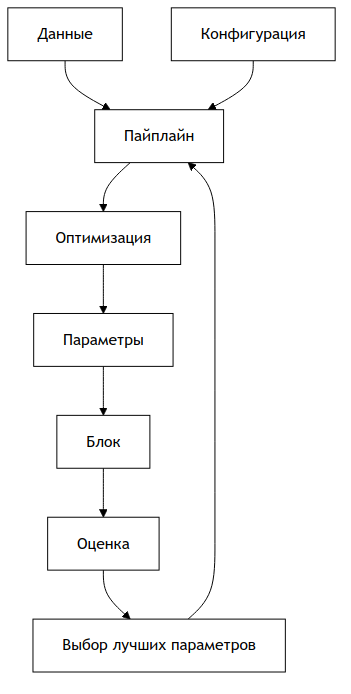
\includegraphics[width=0.6\textwidth,height=0.5\textheight]{img/mermaid/framework_schema.png}
\caption{\label{fig:framework_schema}Схема фреймворка}
\end{figure}
\section{Управление данными}
\label{sec:org98ea497}
Данные в AutoIntent организованы в стандартизованный формат и обрабатываются через специализированный класс Dataset. Исходный набор данных представляет собой JSON или репозиторий на HuggingFace с разбивкой на наборы (например, обучающий (train), валидационный (validation), проверки (test)), где каждая запись содержит текст запроса пользователя (utterance) и метку интента (label). Класс Dataset загружает эти данные и приводит к внутреннему представлению на базе HuggingFace Dataset. При инициализации Dataset автоматически собирается список всех интентов и их описаний, а также проверяется, является ли задача многоклассовой или многолейбловой (мультиметочной).

Для эффективной работы с данными \emph{AutoIntent} использует компонент \emph{DataHandler}, который берёт на себя разделение данных на обучающие и проверочные части согласно настройкам. Параметры разделения задаются в конфигурации \emph{DataConfig}. Например, поле \emph{scheme} определяет схему валидации: значение \texttt{ho} соответствует классическому отложенному набору (\emph{hold-out}), а \texttt{cv} – кросс-валидации. В случае \emph{hold-out}, если входной датасет не содержит явного валидационного-сплита, то \emph{DataHandler} автоматически выделит из обучающих данных долю данных (по умолчанию 20\%) для валидации. Также DataHandler поддерживает режим \emph{few-shot}, когда для обучения используется лишь несколько примеров каждого класса – это бывает полезно при несбаланированом распределении классов. При необходимости DataHandler дополнительно разделяет обучающую выборку между узлами scoring и decision, чтобы избежать утечки данных. При заданном separation\_ratio часть обучающих примеров резервируется для обучения финального классификатора, а остальные – для подбора промежуточных модулей.

Если задана кросс-валидация, \emph{DataHandler} объединяет все обучающие данные и производит стратифицированное разбиение на N под наборов данных (число наборов данных задаётся параметром \emph{n\_folds}, по умолчанию 3). В результате, данные в содержат разбиение на либо train/validation (для hold-out), либо наборы \(train_0, \dots, train_{_(N-1)}\) для кросс-валидации, а также необязательный test (если пользователь предоставил тестовую выборку).
\section{Конфигурация}
\label{sec:org90df4fd}
Весь процесс оптимизации в AutoIntent управляется единым конфигурационным описанием, что гарантирует повторяемость настройки эксперимента и удобство его запуска. Конфигурация задаётся пользователем в виде YAML- или JSON-файла, либо соответствующего Python-словаря, который затем валидируется и загружается с помощью Pydantic-моделей. Основная модель конфигурации – класс \emph{OptimizationConfig} – включает в себя несколько вложенных конфигураций для данных (\emph{DataConfig}), логирования (\emph{LoggingConfig}), параметров моделей (\emph{EmbedderConfig, CrossEncoderConfig, HFModelConfig}), которые будут использоваться если подобные модели не оптимизировалась в рамках подбора параметров, а главное – описание поискового пространства модулей (search\_space). Структура search\_space представляет собой список узлов, для каждого из которых указаны: тип узла (node\_type), целевая метрика оптимизации (target\_metric) и список модулей с набором их гиперпараметров (search\_space внутри узла). Например, в конфигурации можно задать узел типа {}<<scoring>>{} с целевой метрикой F1, в котором рассматриваются два модуля – k-NN с различными значениями k и линейный классификатор с параметрами по умолчанию (см \ref{lst:optimization_config}). Таким образом, конфигурация полностью описывает, какие комбинации методов будут перебраны фреймворком.

\begin{lstlisting}[language=yaml,label=lst:optimization_config,caption={Пример конфигурации},captionpos=b,numbers=none]
- node_type: scoring
  target_metric: scoring_f1
  search_space:
    - module_name: knn
      k:
        low: 1
        high: 20
    - module_name: linear
- node_type: decision
  target_metric: decision_accuracy
  search_space:
    - module_name: argmax
    - module_name: jinoos
\end{lstlisting}

При запуске оптимизации конфигурационный файл считывается и инициализируется объект OptimizationConfig. Далее, на основе полученного конфигурационного объекта инициализируется сам конвейер: создаются оптимизаторы узлов (NodeOptimizer) для каждого описанного узла в поисковом пространстве, а также устанавливаются глобальные параметры (random seed, метод выборки гиперпараметров и так далее).

Пользователь может хранить различные конфигурации для разных датасетов или сценариев и запускать их без изменения кода, просто указывая нужный файл. Каждый эксперимент при запуске сохраняет свою конфигурацию вместе с результатами, что дополнительно гарантирует прозрачность – всегда можно посмотреть, с какими именно параметрами получена та или иная модель.

Для валидации конфигурации используется библиотека Pydantic, которая позволяет задавать типы и ограничения для каждого поля. DatasetConfig, LoggingConfig и другие вложенные конфигурации наследуются от базового класса BaseModel, что позволяют делать проверку корректности сразу.

Для проверки конфигурации модулей во время запуска программы генерируются Pydantic классы для каждого из модулей. Для этого у каждого модуля считываются аннотации типов из метода \texttt{from\_context}, через который все модули инициализируются во время оптимизации. Для более точной валидации были добавлены аннотации \texttt{PositiveInt} и \texttt{FloatFromZeroToOne} для параметров, которые позволяют задать только положительные значения и значения от 0 до 1 соответственно. Это позволяет избежать ошибок при передаче некорректных значений в модули, которые могут привести к сбоям во время работы. Также для каждого числового типа можно задать диапазон значений, что позволяет ограничить поиск только теми значениями (\texttt{low}, \texttt{hight}) и шаг для поиска (\texttt{step}) и \texttt{Literal} для категориальных параметров.

Также для улучшения опыта пользователя генерируется json-схема (JSON Schema) для каждого конфигурационного файла, что позволяет использовать автозаполнение в IDE и проверку типов. Это позволяет избежать ошибок при написании конфигурации и ускоряет процесс настройки эксперимента. Например, если пользователь попытается указать строку вместо числа для параметра k в конфигурации, то IDE выдаст ошибку.
\section{Модули}
\label{sec:org8923aca}
Каждый узел конвейера AutoIntent может быть реализован различными алгоритмическими модулями, что отражает принцип модульности и расширяемости фреймворка. Рассмотрим основные категории узлов и соответствующие им модули.
\subsection{Encoder}
\label{sec:orgd1e957f}
Узел Embedding представляет отвечает за выбор векторизации текста и выполняет промежуточную оценку векторных представлений через два доступных модуля:

\begin{itemize}
\item \emph{RetrievalAimedEmbedding} -- оценивает векторное представление по тому, насколько хорошо оно группирует примеры одного намерения, используя тест \(k\)-NN поиска. Он индексирует обучающие примеры в векторном пространстве (с использованием выбранной модели векторизации) и для каждого выражения из валидационного набора проверяет, содержат ли его \(k\) ближайших соседей правильную метку намерения. Вычисляются такие метрики, как recall, ndcg, map. Более высокий балл указывает на то, что векторизация группирует схожие намерения рядом, что является желаемым для дальнейшей классификации.

\item \emph{LogregAimedEmbedding} -- оценивает векторное представление путем обучения простого классификатора логистической регрессии на векторных представлениях. Он использует модель векторизации для преобразования всех обучающих выражений в векторные признаки, затем обучает логистическую регрессию (опционально с использованием внутренней кросс-валидации для повышения устойчивости). Точность на валидационном наборе (или другая выбранная метрика) этого классификатора отражает, насколько линейно разделимы классы намерений в этом векторном пространстве. Это дает прямой сигнал о полезности векторизации для классификации.
\end{itemize}

Отделяя выбор эмбеддера, AutoIntent избегает повторного обучения тяжелых моделей для каждой попытки классификатора — сначала он находит лучшее текстовое представление (с использованием легких тестов), а затем переиспользует его.
\subsection{Scoring}
\label{sec:orgad1dcb0}
Scoring является главным узлом конвейера, включающим модели машинного обучения, которые непосредственно классифицируют высказывания в намерения. AutoIntent предоставляет богатую коллекцию модулей оценки, каждый из которых реализует различный алгоритм или подход к моделированию для классификации. Во время AutoML оптимизатор оценки будет перебирать различные комбинации этих модулей и их гиперпараметров, чтобы найти лучший вариант. Ключевые модули оценки включают:

\begin{itemize}
\item \emph{KNNScorer} — классификатор на основе метода k ближайших соседей, использующий векторные эмбеддинги. Он использует выбранный эмбеддер для векторизации всех обучающих выражений и хранит их в VectorIndex для эффективного поиска ближайших соседей. Во время предсказания он находит k ближайших обучающих примеров к запросу и вычисляет оценки классов, используя стратегии, такие как равное голосование или метод {}<<ближайшего класса>>{} (каждому классу присваивается кредит от его самого близкого соседа). Это быстрый, непараметрический метод, который часто служит сильной базовой моделью. Его основные гиперпараметры — это k (число соседей) и схема взвешивания, и он зависит от эмбеддера (из узла Embedding) для подачи векторного представления.

\item \emph{LinearScorer} -- линейная модель, которая обучает веса для признаков, чтобы классифицировать намерения. На практике этот модуль  использует логистическую регрессию для обучения на эмбеддингах выражений. Он может иметь гиперпараметры, такие как сила регуляризации. Это полезно как легковесная обучаемая модель — менее мощная, чем глубокие сети, но быстрая и иногда достаточная для простых задач.

\item \emph{SklearnScorer} -- универсальный интерфейс для классификаторов scikit-learn (таких как SVM или случайные леса). Он позволяет легко подключать классические модели машинного обучения. Конкретный алгоритм может быть частью пространства поиска (например, можно попробовать SVM против Наивного Байеса, изменяя параметр).

\item \emph{BertScorer} -- классификатор на основе трансформера с возможностью тонкой настройки. Этот модуль использует трансформер из HuggingFace с головой для классификации. Он будет тонко настраивать трансформер на задаче классификации намерений, создавая мощный классификатор, который часто достигает высокой точности, но требует большего времени на обучение. Гиперпараметры для BertScorer включают такие параметры, как название базовой модели, количество эпох, скорость обучения и так далее, которые AutoIntent может перебирать. Этот модуль олицетворяет нейронную часть спектра в поисковом пространстве.

\item \emph{LoRAScorer} и \emph{PTuningScorer} -- варианты тонкой настройки с параметрической эффективностью. BERTLoRAScorer применяет LoRA (Low-Rank Adaptation) для тонкой настройки трансформера с меньшим числом обучаемых параметров (внедрение обученных матриц адаптации) — это ускоряет обучение и снижает использование памяти. PTuningScorer, вероятно, относится к Prompt Tuning или Prefix Tuning, где обучается небольшая группа эмбеддингов подсказок, в то время как основная модель остается фиксированной. Эти модули позволяют AutoIntent исследовать методы тонкой настройки, которые эффективно используют большие модели на малых данных.

\item \emph{DescriptionScorer} -- подход на основе семантического сходства, использующий описания намерений. Этот модуль использует естественные языковые описания каждого намерения и вычисляет сходство между входным выражением и текстами описаний намерений. Он может работать в двух режимах: в режиме би-энкодера, когда выражение и описание кодируются эмбеддером и сравниваются (например, с использованием косинусного сходства), и в режиме кросс-энкодера, когда пара выражение-описание подается в трансформерную модель (например, модель с перекрестным вниманием), чтобы напрямую вычислить оценку релевантности. В любом случае DescriptionScorer выводит оценку для каждого намерения на основе того, насколько хорошо выражение соответствует описанию намерения, а не на основе примеров из обучающего набора. Это мощный способ работы с намерениями с небольшим количеством примеров или с использованием семантических знаний. Гиперпараметры этого модуля включают выбор между би- или кросс-энкодингом и выбор моделей для каждого из них.

\item \emph{RerankScorer} -- двухступенчатая гибридная модель, которая сочетает извлечение и повторную сортировку с помощью кросс-энкодера. Внутри RerankScorer наследует KNNScorer (проводит начальный поиск соседей), а затем применяет кросс-энкодер для повторной оценки топ-\(m\) соседних результатов. Получив запрос, он находит топ-кандидатов на основе KNN, а затем более точно оценивает этих кандидатов, подавая запрос и каждый пример кандидата в модель кросс-энкодера для получения уточненной оценки сходства. Это повышает точность за счет использования мощной модели на небольшой подмножестве кандидатов, что намного быстрее, чем использование кросс-энкодера для всех намерений или всех обучающих примеров. Гиперпараметры включают \(k\) (для начального извлечения), \(m\) (сколько из них нужно повторно отсортировать, если это отличается от \(k\)).
\end{itemize}

Все эти модули оценки выводят вектор оценок: для заданного выражения они генерируют оценку (или вероятность) для каждого класса намерений. Во время фазы AutoML каждый модуль оценивается путем обучения на обучающем наборе и вычисления одной или нескольких метрик на валидационном наборе через метод score(). Метрики могут включать точность, F1 и т.д., и AutoIntent определяет отдельные функции для метрик для многоклассовых и многозначных случаев, чтобы обеспечить соответствующую оценку. Контекст используется для подачи модулям правильных разделов данных и для сбора результатов. Лучший модуль оценки (с наивысшей метрикой) выбирается для включения в финальный пайплайн. В финальном пайплайне вывода выбранный модуль оценки оборачивается как InferenceNode и будет отвечать за производство оценок для новых выражений. Он взаимодействует с нодой Decision.
\subsection{Decision}
\label{sec:org91b9022}
Узел решения (Decision) – финальный узел, принимающий решение на основе результатов предыдущих шагов. Его задача – вынести окончательный вердикт: один (или несколько) интентов, которые соответствуют запросу пользователя, либо определить, что запрос не относится ни к одному из известных интентов (out-of-scope). Здесь тоже предусмотрено несколько стратегий: Decision является последним этапом пайплайна, который принимает необработанные оценки из нода Scoring и преобразует их в окончательные предсказанные метки для каждого выражения. Этот этап особенно важен для применения порогового отклонения (обнаружение OOS) или выбора нескольких намерений в многозначных сценариях. AutoIntent предлагает несколько модулей принятия решений, все из которых наследуют от BaseDecision:

\begin{itemize}
\item \emph{ArgmaxDecision} -- самая простая стратегия, которая всегда выбирает намерение с наивысшей оценкой в качестве предсказания. Этот модуль выполняет \(prediction = \arg\max score_j\) для каждого выражения. Он не поддерживает OOS (так как всегда выбирает одно из намерений) и используется только для многоклассовой классификации. Этот модуль часто является лучшим выбором, когда OOS не требуется, а оценки классификатора являются надежными вероятностями.

\item \emph{ThresholdDecision} -- конфигурируемый предсказатель на основе порога, который может работать как для многоклассовой, так и для многометочной классификации. Для многоклассовой классификации он выбирает топовое намерение, если его оценка больше некоторого порога \(t\), в противном случае выводит OOS (или {}<<нет намерения>>{}). В многометочной режиме он может применить порог для каждого класса (или вектор порогов), чтобы решить, какие намерения включить в предсказание.
\end{itemize}


\begin{itemize}
\item \emph{JinoosDecision} -- стратегия для многоклассовой классификации с детектированием OOS, в которой порог обнаружения \(T\) выбирается на обучающем наборе путём максимизации метрики
$$j_{in\_oos} = A_{in} + R_{out},$$
где
\begin{itemize}
\item \(A_{in} = \frac{C_{in}}{N_{in}}\) — доля правильно классифицированных не OOS примеров,
\item \(R_{out} = \frac{C_{oos}}{N_{oos}}\) — доля правильно выявленных OOS примеров;
\end{itemize}
при обучении для каждого порога из вычисляются предсказанные классы как \(\arg\max\) и соответствующие им доли уверенности, затем считается \(j_{in\_oos}\) и выбирается порог с наибольшим значением; при предсказании берётся \(\arg\max\) по классам и, если значение уверенности для этого класса ниже \(T\), метка заменяется на OOS, иначе -- индекс класса.

\item \emph{TunableDecision} -- более универсальный модуль оптимизации порога, который работает как для многоклассовой, так и для многометочной классификации и использует Optuna для настройки. В TunableDecision, вместо того чтобы сканировать фиксированную сетку порогов, исследуется набор пороговых значений (один глобальный порог или по одному для каждого класса, в зависимости от сценария), которые максимизируют выбранную целевую метрику. Это эффективно находит оптимальные пороговые значения для каждого класса или в целом, что может значительно улучшить баланс между точностью и полнотой в многометочных задачах или корректно настроить OOS в многоклассовых задачах. TunableDecision поддерживает OOS потенциально обучая порог, который заставляет некоторые низкие оценки восприниматься как отсутствие намерения.

\item \emph{AdaptiveDecision}\autocite{hou_fewshot_2021} -- модуль, предназначенный для многозначной классификации с {}<<адаптивной>>{} стратегией пороговой настройки. Многозначные задачи часто требуют выбора порога для каждого класса, а иногда и их корректировки в зависимости от того, сколько меток нужно предсказать. AdaptiveDecision использует более простой подход, чем полная настройка Optuna: он применяет поиск по коэффициенту масштабирования \(r\), который применяется к стандартным порогам, чтобы оптимизировать метрику (например, F1). Фактически, он может начать с того, что порог каждого класса устанавливается на стандартное значение (например, 0.5) или на основе статистики обучающего набора, а затем находит единственный множитель \(r\), который наилучшим образом регулирует все пороги. AdaptiveDecision не обрабатывает OOS явно. Этот модуль полезен, когда ожидается переменное количество меток и нужно настроить чувствительность.
\end{itemize}

Во время оптимизации конвейера модули \emph{Decision} оцениваются после того, как выбран модуль оценки. На практике, лучшие результаты валидации выбранного модуля \emph{Scoring} (для удержания данных или кросс-валидации) подаются в каждый кандидатный модуль \emph{Decision}, чтобы проверить, насколько хорошо он преобразует оценки в правильные предсказания. Например, после того как классификатор фиксируется, \emph{AutoIntent} может симулировать различные стратегии порогов на его выходных данных, чтобы увидеть, какой из них даст наибольшую точность или F1 на валидации. Целевая метрика для стадии принятия решения может быть такой же, как и для общей метрики (например, если оптимизируется точность конвейера, то будет выбран модуль принятия решения, который дает наибольшую точность на валидации). После выбора модуль принятия решения сохраняется как последняя часть пайплайна. Во время вывода модуль принятия решения просто принимает вектор оценок, выведенный модулем Scoring, и генерирует окончательный набор меток. Эта модульная структура позволяет легко изменять, насколько консервативной или агрессивной будет система при предсказании намерений против OOS, просто изменяя модуль принятия решения (без повторного обучения классификатора).
\section{Обучение}
\label{sec:orgfd353d6}
Оптимизация в контексте AutoIntent представляет собой процесс автоматического подбора оптимальной комбинации модулей и их гиперпараметров для заданного набора данных. Вначале конвейер проверяет, не находится ли он в режиме инференса (то есть, чтобы обучающий метод не был вызван на уже готовом предсказательном конвейере), затем формирует новый Context и настраивает его (данные, логирование, модели если заданы). Далее происходит цикл оптимизации по узлам: AutoIntent проходит последовательно узел за узлом в определённом порядке (сначала embedding, потом scoring и в конце decision), запускает для каждого соответствующий NodeOptimizer и ждёт, пока он подберёт лучший модуль для своего этапа.

Процесс внутри NodeOptimizer построен на использовании библиотеки Optuna\autocite{akiba_optuna_2019a} для эффективного исследования пространства параметров. Каждому узлу соответствует список модулей-кандидатов (из конфигурации search\_space), и для каждого модуля задан диапазон значений гиперпараметров. Затем оптимизатор осуществляет вложенный цикл: перебирает модули по очереди и для каждого выполняет серию испытаний с разными комбинациями гиперпараметров. Методология перебора задаётся параметром sampler – AutoIntent поддерживает несколько стратегий: \texttt{brute} (полный перебор всех комбинаций, если их число невелико), \texttt{random} (случайный поиск фиксированного числа итераций) и \texttt{tpe} (алгоритм Tree-Structured Parzen Estimator из Optuna для байесовской оптимизации). По умолчанию используется brute-force, однако для непрерывных или обширных пространств целесообразно переключиться на более умные подходы.

Внутри одного испытания NodeOptimizer выполняет следующие шаги. Сначала на основе текущих значений гиперпараметров создаётся конфигурация модуля через Optuna, которая подбирает значения в зависиомости от стратегии. Затем создаётся экземпляр класса модуля с заданными параметрами, при необходимости дополняются имплицитные параметры (в некоторых модулях, например, может вычисляться размер выходного слоя на основе данных), и модуль тренируется/применяется на обучающих данных из Context и выдает предсказания на валидационном наборе. Целевое значение извлекается и возвращается Optuna, которая на основании него принимает решение о выборе следующей комбинации гиперпараметров. Параллельно, вся информация о проведённом испытании фиксируется. AutoIntent логирует параметры модуля, полученные метрики, возможные артефакты, а также немедленно сохраняет обновлённый прогресс на диск. Это позволяет даже в случае прерывания эксперимента иметь данные о уже проверенных комбинациях и, при надлежащих настройках, потом восстановиться и продолжить поиск.

После того, как все узлы оптимизированы, AutoIntent формирует финальный конвейер (inference). На этом шаге классы-оптимизаторы узлов (NodeOptimizer) заменяются на соответствующие им инференс-обёртки (InferenceNode), содержащие внутри уже настроенные лучшие модули. Конвейер обновляет свой список узлов: вместо множества пробуемых модулей фиксируется по одному выбранному модулю на узел.
\section{Aугментация}
\label{sec:orga4f9b5e}
Также разработан модуль для расширения (аугментации) набора данных. Он состоит из нескольких взаимосвязанных компонентов, предназначенных для генерации новых обучающих данных. Сейчас разработано несколько способов для расширения набора данных. Сейчас разработаны 3 механизма расширения данных: базовая генерация, инкрементальная с учетом качества и адаптация с помощью DSPY\autocite{khattab_dspy_2023}.

Метод базовой генерации в опирается на синтез-шаблоны, которые формируют промпт, содержащий название интента и примеры существующих высказываний, затем запрашивают у языковой модели новые фразы. В процессе подготовки промпта шаблон извлекает до пяти примеров каждого интента, и просит {}<<сгенерировать N дополнительных примеров>>{}.

Инкрементальное расширение данных объединяет порождение парафраз с непрерывным контролем эффективности конвейера: на каждом раунде он генерирует по одному новому варианту текста для каждого высказывания, добавляет их во временный набор данных и обучает {}<<быстрый>>{} конвейер. После оценки на валидационных данных сравниваются текущая точность с лучшей из предыдущих итераций; если качество повышается, новые образцы сохраняются и цикл повторяется, иначе последний раунд отбрасывается, а процесс останавливается. Это обеспечивает остановку аугментации ровно в тот момент, когда она перестаёт приносить улучшение модели.

Используя возможности DSPy для оптимизированного поиска парафраз вместо ручных шаблонов определяется DSPy задача {}<<парафразирования текста>>{}, а итеративный оптимизатор \emph{MiPROv2}\autocite{opsahl-ong_optimizing_2024} (\emph{Multiprompt Instruction PRoposal Optimizer Version 2}) генерирует кандидатов и оценивает их по комбинированной метрике — семантического сходства с учётом штрафа ROUGE-1\autocite{lin_rouge_} за прямое копирование. Лучшие предложения отбираются автоматически, после чего их влияние на конвейер проверяется аналогично инкрементальному улучшение. Такой подход минимизирует ручное конструирование промптов и фокусируется на нахождении наилучших по качеству и разнообразию примеров.
\section{Логирование}
\label{sec:orgd1f8846}
В процессе работы AutoIntent ведёт два уровня логов: системные (через стандартный модуль logging Python) и встраивание модулей для обработки вызовов (через \emph{CallbackHandler}). В системные логи выводятся информационные сообщения о ходе оптимизации, предупреждения о потенциальных некорректных настройках и прочие служебные сведения – они, как правило, сохраняются в текстовый файл в папке запуска. Метрики обрабатываются CallbackHandler: при старте каждого прогона модуля открывает новый эксперимент в системе мониторинга, а далее для каждого эксперимента вызываются затем при старте и конце каждого модуля и в конце сохраняются финальные метрики. Сейчас добавлены 2 модуля для сохранения метрик во внешние сервисы: TesnsorBoard и WandDB\footnote{\url{https://wandb.ai/}}.
\chapter{Эксперименты}
\label{sec:org349a146}
\section{Наборы данных для сравнения}
\label{sec:orgc532320}
Для оценки точности, надёжности и масштабируемости методов определения пользовательских намерений были отобраны шесть признанных наборов данных: Banking77\autocite{casanueva_efficient_2020}, MINDS-14\autocite{gerz_multilingual_2021}, HWU64\autocite{liu_benchmarking_2019}, SNIPS\autocite{coucke_snips_2018}, MASSIVE\autocite{fitzgerald_massive_2022} и CLINC150\autocite{unknown_clinc150_2020}. Эти наборы данных представляют разнообразие доменов (от банковских запросов до общих ассистентов) и включают «out-of-scope» примеры, что обеспечивает всестороннюю проверку алгоритмов определения намерений пользователей.
\section{Анализ модуля оценки}
\label{sec:org1eeb21c}
Была проведена оценка модулей с использованием моделей по-умолчанию нашего фреймворка (\emph{prajjwal1/bert-tiny}\autocite{bhargava_generalization_2021} в качестве \emph{Bert} и \emph{sentence-transformers/all-MiniLM-L6-v2} для \emph{SentneceTransformer}). Экспериментальная настройка включала отложенную валидацию и оптимизацию гиперпараметров с полным перебором (параметры запуска \ref{src:light_backbone}).

Результаты, представленные в таблице \ref{tbl:light_modules}, выявляют несколько ключевых закономерностей. Логистическая регрессия на основе трансформерных эмбеддингов ({}<<linear>>{} в таблице) показывает наилучшие результаты как по средней точности, так и по устойчивости работы на разных наборах данных, достигая высшей оценки в трёх из пяти наборов. Методы на базе BERT демонстрируют значительную вариативность результатов: параметро-эффективные подходы (P-tuning и LoRA) существенно уступают, полная тренировка BERT даёт конкурентоспособные результаты лишь на одном наборе, в то время как на остальных показывает более низкую точность. Это указывает на возможные трудности в оптимизации гиперпараметров для методов, основанных на тренировке. Методы zero-shot (логистическая регрессия, KNN) стабильно превосходят трансформерные подходы, при этом все три демонстрируют среднюю точность выше 90 \%.

\begin{table}[h!]
\caption{\label{tbl:light_modules}Доля правильных ответов модулей оценки с параметрами по-умолчанию}
\centering
\begin{tabular}{|p{2cm}|p{2cm}|p{2cm}|p{2cm}|p{2cm}|p{2cm}|p{2cm}|}
\hline
 & Banking77 & MINDS-14 & HWU64 & SNIPS & MASSIVE & Среднее\\
\hline
PTuning & 4.63 & 11.63 & 3.65 & 66.49 & 8.57 & 18.99\\
\hline
LoRA & 20.35 & 12.40 & 22.40 & 95.09 & 41.95 & 38.44\\
\hline
BERT & 64.14 & 69.77 & 73.40 & \uline{98.52} & 76.76 & 76.52\\
\hline
Rerank & 89.04 & \uline{97.67} & 84.45 & 96.59 & 81.68 & 89.89\\
\hline
kNN & 89.74 & \uline{97.67} & 85.42 & 96.10 & 81.65 & 90.12\\
\hline
Linear & \uline{90.51} & \uline{97.67} & \uline{89.17} & 97.45 & \uline{84.70} & \uline{91.90}\\
\hline
\end{tabular}
\end{table}
Для изучения влияния ёмкости модели на качество классификации мы повторили эксперименты с более большими трансформерами (\emph{microsoft/deberta-v3-small}\autocite{he_debertav3_2023} для \emph{BERT} и \emph{mixedbread-ai/mxbai-embed-large-v1}\autocite{li_angleoptimized_2024} в качестве \emph{SentenceTransformer}). Несмотря на то, что общий рейтинг по средней точности остался согласован с результатами для лёгких моделей, изменилось распределение лидирующих методов по отдельным наборам данных. Преимущество логистической регрессии стало менее выраженным: KNN показал сопоставимые показатели числа {}<<выигрышей>>{} на отдельных выборках. Методы на базе BERT по-прежнему отстают от методов на основе признаков, хотя полная тренировка BERT продемонстрировала улучшенные результаты на некоторых наборах. Это свидетельствует о том, что лишь увеличение ёмкости модели может быть недостаточно для преодоления сложностей оптимизации трансформерных методов. Конкурентоспособность нескольких методов на основе признаков оправдывает включение разнообразных модулей оценки в библиотеку, особенно для приложений, где критически важно выявление оптимальной модели.

\begin{table}[h!]
\caption{\label{tbl:heavy_modules}Производительность модулей оценки с более большими моделями}
\centering
\begin{tabular}{|p{2cm}|p{2cm}|p{2cm}|p{2cm}|p{2cm}|p{2cm}|p{2cm}|}
\hline
 & Banking77 & MINDS-14 & HWU64 & SNIPS & MASSIVE & Среднее\\
\hline
PTuning & 5.00 & 14.73 & 9.64 & 91.67 & 25.87 & 29.38\\
\hline
LoRA & 13.82 & 9.30 & 38.58 & 99.13 & 52.06 & 42.58\\
\hline
BERT & 85.61 & 48.06 & 88.58 & \uline{99.16} & 86.36 & 81.56\\
\hline
Rerank & 90.28 & 96.12 & 87.24 & 97.35 & 83.87 & 90.97\\
\hline
kNN & \uline{92.14} & \uline{98.45} & 89.43 & 96.97 & 85.43 & 92.48\\
\hline
Linear & 91.81 & 96.90 & \uline{91.78} & 98.06 & \uline{87.58} & \uline{93.23}\\
\hline
\end{tabular}
\end{table}
\section{Анализ качества работы в зависимости от базовой модели}
\label{sec:orga25ad68}
Для оценки влияния базовой модели на производительность модулей оценки была проведена серия экспериментов с различными предобученными моделями. Были выбраны модели до 1 миллиарда параметров, которые занимали высокие места на \emph{MTEB(eng, v2)}\autocites{muennighoff_mteb_2023}[][]{enevoldsen_mmteb_2025}, также были добавлены модели deberta для сравнения качества с предыдущими экспериментами.

Было проведено 2 серии экспериментов: в первой серии использовался фиксированный модуль эмбеддинга и лучшие модели считались на финальном этапе конвейера по точности предсказанных классов (accuracy)\ref{tbl:embedding_models_accuracy} (конфигурация \ref{src:encoder_config}), а во втором модели перебирались на узле \emph{Embedding} и модели выбирались по лучшему NDCG\ref{tbl:embedding_models_ndcg}.

Как можно увидеть из таблиц, лучшее качество показала модель \texttt{NovaSearch/stella\_en\_400M\_v5}\autocite{zhang_jasper_2025}, а остальные модели оказались на сопоставимом уровне. Это показывает, что в целом для данных можно перебрать предобученные модели на узле \emph{Embedding} и получить сопоставимое качество, что и перебирать модели отдельно.
\section{Базовые сравнения}
\label{sec:org510f5eb}

В этом разделе приводится сравнительный анализ качества классификации, измеренного в процентах точности (accuracy), для нашего фреймворка AutoIntent и четырёх популярных открытых AutoML-решений: LightAutoML, FEDOT, H2O и AutoGluon. Эксперименты проводились на пяти публичных датасетах для задачи распознавания намерений пользователя — Banking77, HWU64, MASSIVE, MINDS14 и SNIPS. Результаты по каждому фреймворку и датасету, а также усреднённое значение точности, представлены в таблице \ref{tbl:frameworks_comparison}.

Сравнение AutoIntent с открытыми NLP AutoML-фреймворками:

\begin{table}[h!]
\caption{\label{tbl:frameworks_comparison}Сравнение производительности AutoML-фреймворков}
\centering
\begin{tabular}{|p{3cm}|p{2cm}|p{2cm}|p{2cm}|p{2cm}|p{1cm}|p{2cm}|}
\hline
 & Banking77 & HWU64 & MASSIVE & MINDS14 & SNIPS & Среднее\\
\hline
LightAutoML & 1.30 & 1.77 & 7.04 & 8.33 & 14.50 & 6.59\\
\hline
FEDOT & 1.30 & 1.77 & 7.28 & 12.04 & 15.14 & 7.51\\
\hline
H2O & 75.32 & 77.32 & 75.30 & 76.85 & 98.36 & 80.63\\
\hline
AutoGluon & 93.28 & 91.17 & 88.92 & 97.22 & 99.07 & 93.13\\
\hline
AutoIntent & 92.86 & 90.83 & 87.13 & 95.68 & 98.19 & 92.94\\
\hline
\end{tabular}
\end{table}

Как видно из таблицы, общая картина распределения качества классификации чётко выделяет две группы фреймворков. LightAutoML и FEDOT оказываются не готовыми для задач распознавания диалоговых намерений, демонстрируя результаты ниже 10 \% на трёх из пяти датасетов. H2O, в свою очередь, стабильно удерживается на уровне около 75–77 \%, что значительно лучше базовых решений, но всё же не дотягивает до показателей современных AutoML-систем. Лидерами выступают AutoGluon и AutoIntent: AutoGluon занимает первое место с средним значением точности 93.13 \%, тогда как AutoIntent лишь на 0.19 \% отстаёт и показывает 92.94 \% в среднем по всем бенчмаркам.

При более детальном рассмотрении по датасетам разница между AutoGluon и AutoIntent не превышает 1.8 процентного пункта даже в наименее удачном для нашего фреймворка наборе MASSIVE, а в большинстве случаев разрыв составляют менее 1 \%. Это демонстрирует, что AutoIntent способен конкурировать с ведущими решениями на рынке, обеспечивая практически сопоставимое качество.
\subsection{Детектирование вне области (OOS)}
\label{sec:org4404b69}

Для сравнения возможностей обнаружения OOS был использован набор данных CLINC150, адаптировав все фреймворки без встроенной OOS-поддержки путём добавления OOS как отдельного класса. Базовые решения FEDOT и LightAutoML показали нулевую точность в распознавании {}<<в области>>{} (in\_domain\_acc = 0 \%), при этом их точность детекции OOS составила лишь 18.18 \%, хотя полнота оказалась максимальной (oos\_recall = 100 \%). Это говорит о том, что они полностью игнорируют обычные классы намерений и метят всё как {}<<вне области>>{}.

Фреймворки H2O, AutoGluon и AutoIntent продемонстрировали более зрелый подход. H2O добился 85.22 \% точности в распознавании «в области», при приемлемой 82.57 \% точности OOS, однако полнота детекции «вне области» оказалась низкой — всего 27 \%. AutoGluon показал лучший баланс: 95.76 \% в рамках домена и высокую OOS точность (98.47 \%), но всё же низкую полноту — 32.20 \%. Наконец, AutoIntent продемонстрировал наилучшую полноту обнаружения OOS (65.93 \%) при высокой точности в домене (96.13 \%) и точности OOS 91.92 \%, что делает его наиболее сбалансированным решением для задач с непредвиденными запросами.

\begin{table}[h!]
\caption{\label{tbl:oos_detection}Результаты OOS-детектирования}
\centering
\begin{tabular}{|p{3cm}|p{2cm}|p{2cm}|p{2cm}|}
\hline
 & in\_domain\_acc & oos\_precision & oos\_recall\\
\hline
FEDOT & 0.00 & 18.18 & 100.00\\
\hline
LightAutoML & 0.00 & 18.18 & 100.00\\
\hline
H2O & 85.22 & 82.57 & 27.00\\
\hline
AutoGluon & 95.76 & 98.47 & 32.20\\
\hline
AutoIntent & 96.13 & 91.92 & 65.93\\
\hline
\end{tabular}
\end{table}
\subsection{Качество классификации в условиях малого числа примеров}
\label{sec:org103f2ae}
В условиях дисбаланса классов и ограниченного объёма разметки возникает задача оценки качества классификации при малом числе примеров на класс, или «few-shot» обучении. Такие сценарии характерны для новых доменов или редких пользовательских намерений, когда собрать крупный обучающий набор сложно или дорого. В данном разделе мы проводим серию экспериментов постепенно увеличивая количество примеров (shots) от 4 до полного тренировочного набора, и сравниваем, как AutoIntent, AutoGluon и H2O реагируют на увеличение объёма обучающих данных в условиях few-shot.

\begin{figure}[h!]
\centering
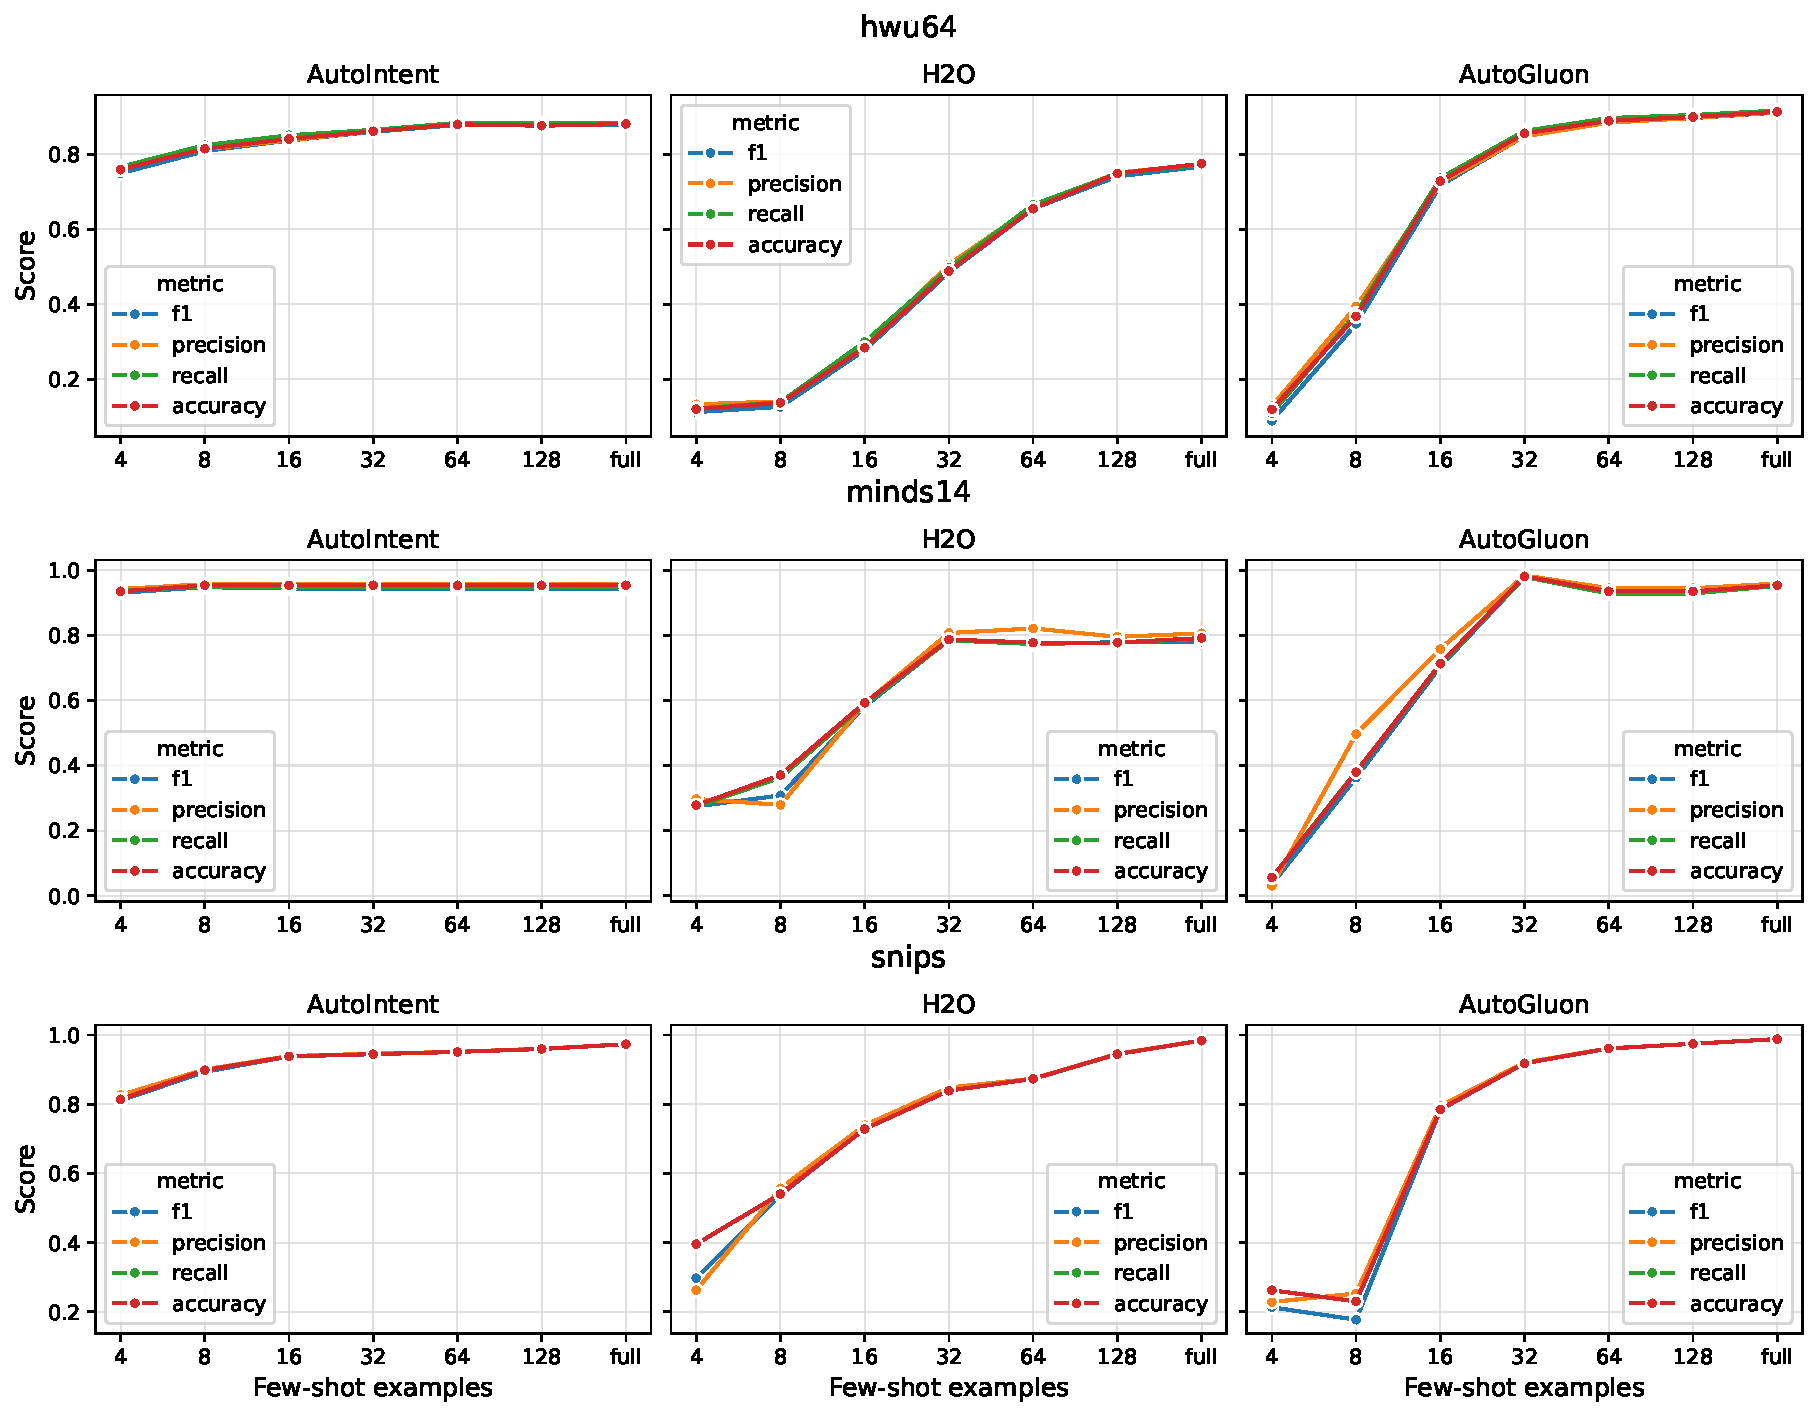
\includegraphics[width=0.8\textwidth]{img/comparison_few_shot_subfigures.pdf}
\caption{\label{fig:few_shot_comparison}Сравнение качества классификации в условиях few-shot обучения}
\end{figure}

По результатам экспериментов видно (см рисунок \ref{fig:few_shot_comparison} и таблицу \ref{tbl:few_shot_comparison}), что при очень ограниченном наборе примеров (4–8 shots) AutoIntent существенно опережает как AutoGluon, так и H2O. Уже при 4 примерах средняя точность AutoIntent достигает 0.76 на HWU64, 0.94 на MINDS14 и 0.81 на SNIPS, тогда как AutoGluon едва превосходит 0.12, 0.06 и 0.26 соответственно, а H2O колеблется между 0.12 и 0.40. При увеличении до 8 примеров AutoIntent выходит на 0.82–0.95, в то время как AutoGluon лишь до 0.23–0.38, а H2O до 0.14–0.54. Это демонстрирует, что наш фреймворк максимально эффективно использует каждый дополнительный пример, обеспечивая быструю наращиваемость качества классификации в режимах few-shot.

С ростом числа примеров до 16–32 shots разрыв между AutoIntent и AutoGluon сокращается: при 16 shots AutoIntent показывает 0.84–0.95 против 0.73–0.79 у AutoGluon, а при 32 shots оба фреймворка достигают примерно одинаковых 0.86–0.95 (кроме незначительного преимущества AutoGluon на MINDS14). H2O отстаёт на 0.49–0.84. При дальнейшем увеличении до 64–128 примеров и использовании полного датасета все системы выходят на «плато» производительности: AutoGluon стабилизируется на 0.89–0.91, AutoIntent – на 0.88–0.97, H2O – на 0.66–0.98. AutoIntent сохраняет высокую точность, максимально приближаясь к лидеру AutoGluon, но при этом достигает сопоставимых результатов уже при меньших объёмах обучающих данных.
\section{Расширение набора данных}
\label{sec:org77879df}
Для моделирования практических ситуаций с ограниченным объёмом разметки мы сформировали случайные 10-shot версии пяти датасетов. Такой подход показывает, как пользователи могут расширять минимальные обучающие наборы данных синтетическими примерами. Были протестированы четыре LLM (\emph{DeepSeek-V3-0324}\autocite{deepseek-ai_deepseekv3_2025}, \emph{GPT-4o-mini}\autocite{openai_gpt4o_2024}, \emph{Qwen2.5-7B}\autocite{yang_qwen2_2024}, \emph{Llama-3.1-8B}\autocite{dubey_llama_2024}) на английских (Banking77, SNIPS), русскоязычных (Banking77ru, SNIPSru) и с OOS (Clinc150) наборах данных.

Корреляционный анализ (см. таблицы \ref{tbl:corr_analisys}, \ref{tbl:augmented_models_performance}) выявил несколько ключевых закономерностей.
\begin{figure}[h!]
\centering
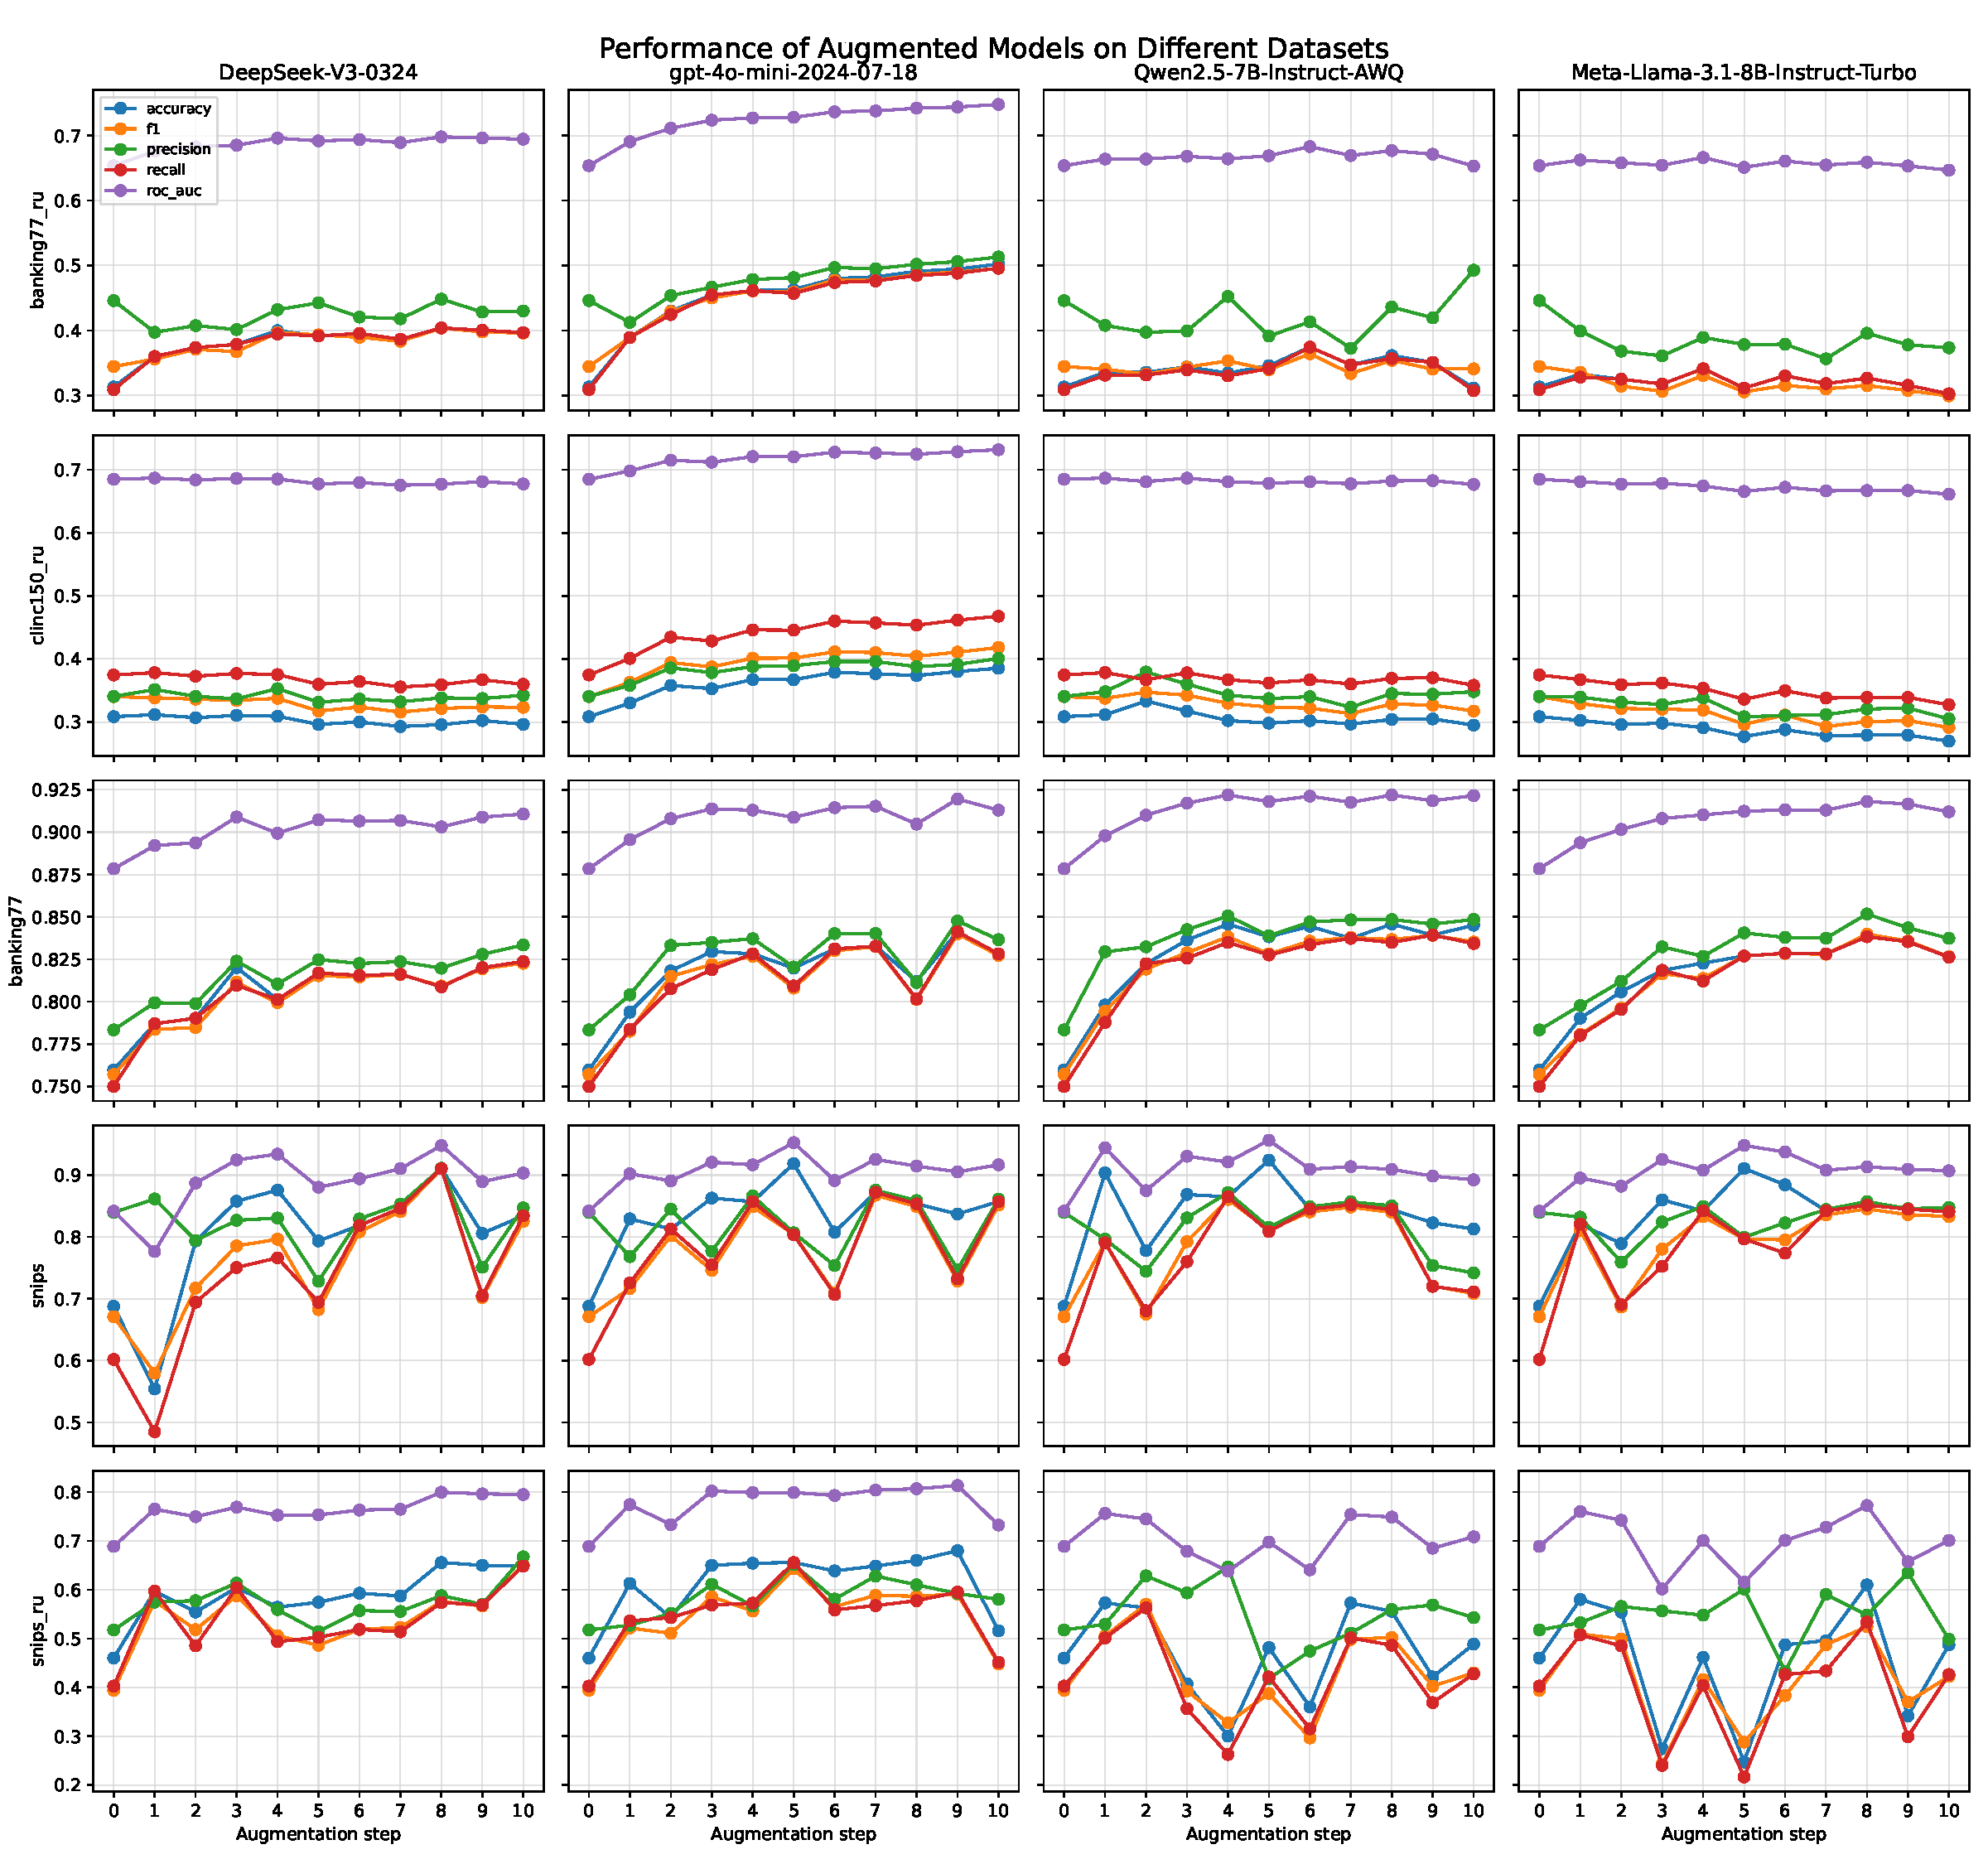
\includegraphics[width=0.8\textwidth]{img/augmented_models_performance.pdf}
\caption{\label{fig:augmented_models_performance}Сравнение качества по шагам аугментации}
\end{figure}


Неожиданно, ни размер, ни тип модели (проприетарная или open-source) не коррелировали однозначно с эффективностью аугментации. И более компактные Llama-3.1-8B, и крупные DeepSeek-V3-0324 демонстрировали схожие профили улучшения.

Эти результаты указывают на то, что эффективность расширения данных мало зависит от конкретной LLM, однако GPT-4o-mini показал наиболее стабильный положительный эффект. Англоязычные датасеты в целом выигрывают от аугментации сильнее, чем их русскоязычные аналоги — вероятно, из-за ориентированности наших промптов на английский язык. При этом производительность OOS-детекции имеет тенденцию к снижению с ростом числа синтетических примеров, особенно для CLINC150\_ru: сочетание высокой гранулярности (150 классов) и универсального характера синтетики плохо передаёт тонкие границы между классами. Наиболее стабильное улучшение OOS-метрик при любом объёме добавления наблюдалось на banking77.
\begin{table}[h!]
\caption{\label{tbl:corr_analisys}Корреляционный анализ (значения r, незначимые опущены)}
\centering
\begin{tabular}{|p{4cm}|p{2cm}|p{2cm}|}
\hline
Model & English & OOS\\
\hline
DeepSeek-V3-0324 & 0.532 & -0.777\\
\hline
gpt-4o-mini-2024-07-18 & 0.500 & 0.884\\
\hline
Qwen2.5-7B-Instruct-AWQ & – & -0.613\\
\hline
Meta-Llama-3.1-8B-Instruct-Turbo & 0.568 & -0.932\\
\hline
\end{tabular}
\end{table}

Для дальнейшего изучения влияния аугментации на качество классификации мы провели подробный статистический анализ изменений точности до и после расширения данных на каждом уровне (от 1 до 10 синтетических образцов). Были выполнены попарные t-тесты для оценки статистической значимости и рассчитаны величины эффекта с помощью коэффициента Коуэна (Cohen’s d) (табл. 7).

\begin{table}[h!]
\caption{\label{tbl:augmented_models_performance}Результаты анализа до и после аугментации}
\centering
\begin{tabular}{|p{1cm}|p{1.5cm}|p{1.5cm}|p{1.5cm}|p{2.5cm}|}
\hline
naug & T-stat & P & Эффективный размер & Среднее улучшение\\
\hline
1 & 3.736 & 0.002 & 0.355 & 0.071\\
\hline
2 & 8.399 & 2.934e-07 & 0.366 & 0.072\\
\hline
3 & 3.280 & 0.005 & 0.331 & 0.078\\
\hline
4 & 3.875 & 0.001 & 0.365 & 0.083\\
\hline
5 & 3.247 & 0.005 & 0.351 & 0.086\\
\hline
6 & 4.990 & 0.000 & 0.408 & 0.088\\
\hline
7 & 6.751 & 4.652e-06 & 0.470 & 0.100\\
\hline
8 & 7.389 & 1.531e-06 & 0.567 & 0.117\\
\hline
9 & 4.088 & 0.001 & 0.389 & 0.086\\
\hline
10 & 5.633 & 3.743e-05 & 0.406 & 0.087\\
\hline
\end{tabular}
\end{table}
Результаты анализа:
\begin{enumerate}
\item Любой уровень аугментации (1–10 примеров) даёт статистически значимые улучшения (p < 0.01) по сравнению с базой без аугментации.
\item Коэффициенты Коуэна варьируются от 0.33 до 0.57, что соответствует средним и крупным практическим эффектам.
\item Средний прирост точности растёт вместе с числом синтетических примеров: от 7.1 \% при единичном добавлении до 11.7 \% при максимальном. При этом наблюдается раннее насыщение — темпы прироста замедляются после 4–6 примеров.
\end{enumerate}

Таким образом, LLM-расширение данных обеспечивает не только статистически значимые, но и практически ощутимые улучшения качества классификации, а оптимальным диапазоном генерации синтетических примеров считается 4–8 на класс.
\chapter*{Заключение}
\label{sec:org8e735e7}
\addcontentsline{toc}{chapter}{Заключение}
В ходе работы был спроектирован и разработан фреймворк для автоматического определения пользовательских намерений. Проведён глубокий анализ современных подходов к классификации намерений, включая обзор существующих библиотек и алгоритмов машинного обучения, что позволило выявить потребность в инструменте, способном адаптироваться к самым разным предметным областям без постоянного вмешательства эксперта. На основе полученных данных разработана модульная архитектура автоматического выбора моделей и гиперпараметров, а также комплексных процедур оценки их качества.

Экспериментальная часть работы показала, что автоматический подбор моделей и параметров обеспечивает прирост точности классификации. Сравнительный анализ продемонстрировал, что разработанное решение сопоставимо или превосходит по качеству аналогичные фреймворки при минимальных усилиях разработчика, что подчёркивает его практическую значимость.

\printbibliography[title=СПИСОК\spaceИСПОЛЬЗОВАНЫХ\spaceИСТОЧНИКОВ]
\appendix
\chapter*{ПРИЛОЖЕНИЕ А. Конфигурации}
\label{sec:orga9676c5}
\addcontentsline{toc}{chapter}{ПРИЛОЖЕНИЕ А. Конфигурации}
\begin{lstlisting}[language=yaml,label=src:light_backbone,caption={Параметры для сравнения модулей с параметрами по-умолчанию},captionpos=b,numbers=none]
- node_type: scoring
  target_metric: scoring_accuracy
  metrics: [scoring_roc_auc, scoring_precision, scoring_recall, scoring_f1]
  search_space:
    - module_name: knn
      n_trials: 5
      k:
        low: 1
        high: 20
      weights: [uniform, distance, closest]
    - module_name: linear
    - module_name: dnnc
      n_trials: 5
      k:
        low: 1
        high: 5
    - module_name: rerank
      k: [5]
      weights: [uniform, distance]
      m: [ 1, 2, 3, 4, 5 ]
      use_crosencoder_scores: [True, False]
    - module_name: sklearn
      n_trials: 5
      clf_name: [RandomForestClassifier]
      n_estimators: [200, 300, 500]
      max_depth: [100, 150, 200]
      max_features: [sqrt, log2, null]
    - module_name: bert
      n_trials: 5
      num_train_epochs: [3]
      batch_size: [8, 16, 32]
      learning_rate: [5.0e-5, 1.0e-4, 5.0e-4, 1.0e-3]
    - module_name: lora
      n_trials: 5
      num_train_epochs: [3]
      batch_size: [8, 16, 32]
      learning_rate: [5.0e-5, 1.0e-4, 5.0e-4, 1.0e-3]
      lora_alpha: [16, 32, 64]
      lora_dropout: [0.1, 0.2, 0.3]
      r: [8, 16, 32, 64]
    - module_name: ptuning
      n_trials: 5
      num_train_epochs: [3]
      batch_size: [8, 16, 32]
      learning_rate: [5.0e-5, 1.0e-4, 5.0e-4, 1.0e-3]
      num_virtual_tokens: [10, 30, 50]
      encoder_dropout: [0.1, 0.2, 0.3]
      encoder_hidden_size: [128, 256, 512]
      encoder_reparameterization_type: [MLP, LSTM]
      encoder_num_layers: [1, 2, 3]
- node_type: decision
  target_metric: decision_accuracy
  search_space:
    - module_name: argmax
\end{lstlisting}

\begin{lstlisting}[language=yaml,label=src:encoder_config,caption={Параметры для сравнения различных моделей эмбеддинга},captionpos=b,numbers=none]
- node_type: embedding
  target_metric: retrieval_ndcg
  metrics:
    - retrieval_hit_rate
    - retrieval_map
    - retrieval_mrr
    - retrieval_ndcg
    - retrieval_precision
  search_space:
    - module_name: retrieval
      k: [10]
- node_type: scoring
  target_metric: scoring_roc_auc
  search_space:
    - module_name: knn
      k:
        - 5
        - 10
      weights:
        - distance
    - module_name: linear
- node_type: decision
  target_metric: decision_accuracy
  search_space:
    - module_name: threshold
    - module_name: tunable
    - module_name: argmax
    - module_name: jinoos
\end{lstlisting}

\begin{lstlisting}[language=yaml,label=src:few_shot_config,caption={Параметры для few-shot обучения},captionpos=b,numbers=none]
- node_type: scoring
  target_metric: scoring_accuracy
  metrics: [scoring_roc_auc, scoring_precision, scoring_recall, scoring_f1]
  search_space:
    - module_name: knn
      n_trials: 20
      k:
        low: 1
        high: 20
      weights: [uniform, distance, closest]
    - module_name: linear
    - module_name: dnnc
      k:
        low: 1
        high: 5
- node_type: decision
  target_metric: decision_accuracy
  search_space:
    - module_name: argmax
    - module_name: threshold
      thresh:
        low: 0.1
        high: 0.9
        step: 0.1
    - module_name: jinoos
\end{lstlisting}
\chapter*{ПРИЛОЖЕНИЕ Б. Таблицы сравнения моделей}
\label{sec:org3bca429}
\addcontentsline{toc}{chapter}{ПРИЛОЖЕНИЕ Б. Таблицы сравнения моделей}

\begin{table}[h!]
\caption{\label{tbl:embedding_models_accuracy}Результативность различных моделей эмбеддинга (accuracy)}
\centering
\begin{tabular}{|p{5cm}|p{2cm}|p{2cm}|p{2cm}|p{2cm}|p{2cm}|}
\hline
 & HWU64 & MASSIVE & MINDS14 & SNIPS & Среднее\\
\hline
NovaSearch/stella-en-400M-v5\autocite{zhang_jasper_2025} & \uline{0.92} & \uline{0.89} & 0.97 & 0.98 & \uline{0.94}\\
\hline
intfloat/multilingual-e5-large-instruct\autocite{wang_multilingual_2024} & 0.91 & 0.87 & \uline{0.98} & 0.98 & 0.94\\
\hline
avsolatorio/GIST-large-Embedding-v0\autocite{solatorio_gistembed_2024} & 0.91 & 0.88 & 0.97 & 0.98 & 0.94\\
\hline
WhereIsAI/UAE-Large-V1\autocite{li_angleoptimized_2024} & 0.91 & 0.87 & 0.95 & 0.98 & 0.93\\
\hline
BAAI/bge-m3\autocite{chen_bge_2024} & 0.91 & 0.87 & 0.94 & \uline{0.99} & 0.93\\
\hline
intfloat/multilingual-e5-large\autocite{wang_multilingual_2024} & 0.89 & 0.84 & 0.94 & 0.98 & 0.91\\
\hline
sentence-transformers/LaBSE & 0.88 & 0.84 & 0.92 & 0.98 & 0.90\\
\hline
HIT-TMG/KaLM-embedding-multilingual-mini-instruct-v1.5\autocite{hu_kalmembedding_2025} & 0.88 & 0.83 & 0.96 & 0.91 & 0.90\\
\hline
nomic-ai/nomic-embed-text-v1.5\autocite{nussbaum_nomic_2025} & 0.80 & 0.78 & 0.95 & 0.96 & 0.87\\
\hline
microsoft/deberta-v3-small & 0.77 & 0.77 & 0.73 & 0.98 & 0.81\\
\hline
microsoft/deberta-v3-large & 0.70 & 0.69 & 0.66 & 0.97 & 0.75\\
\hline
microsoft/deberta-v3-base & 0.69 & 0.72 & 0.63 & 0.96 & 0.75\\
\hline
\end{tabular}
\end{table}

\begin{table}[h!]
\caption{\label{tbl:embedding_models_ndcg}Результативность различных моделей эмбеддинга (NDCG)}
\centering
\begin{tabular}{|p{5cm}|p{2cm}|p{2cm}|p{2cm}|p{2cm}|p{2cm}|}
\hline
 & HWU64 & MASSIVE & MINDS14 & SNIPS & Среднее\\
\hline
NovaSearch/stella-en-400M-v5 & \uline{0.92} & \uline{0.89} & 0.97 & \uline{0.98} & \uline{0.94}\\
\hline
avsolatorio/GIST-large-Embedding-v0 & 0.91 & 0.88 & 0.97 & 0.97 & 0.93\\
\hline
WhereIsAI/UAE-Large-V1 & 0.91 & 0.88 & 0.97 & 0.97 & 0.93\\
\hline
intfloat/multilingual-e5-large-instruct & 0.91 & 0.87 & 0.97 & 0.98 & 0.93\\
\hline
HIT-TMG/KaLM-embedding-multilingual-mini-instruct-v1.5 & 0.89 & 0.86 & \uline{0.99} & 0.96 & 0.93\\
\hline
BAAI/bge-m3 & 0.89 & 0.87 & 0.96 & 0.97 & 0.92\\
\hline
intfloat/multilingual-e5-large & 0.89 & 0.86 & 0.97 & 0.98 & 0.92\\
\hline
nomic-ai/nomic-embed-text-v1.5 & 0.84 & 0.82 & 0.96 & 0.95 & 0.90\\
\hline
sentence-transformers/LaBSE & 0.86 & 0.85 & 0.89 & 0.98 & 0.90\\
\hline
microsoft/deberta-v3-small & 0.58 & 0.60 & 0.57 & 0.93 & 0.67\\
\hline
microsoft/deberta-v3-large & 0.54 & 0.54 & 0.41 & 0.90 & 0.60\\
\hline
microsoft/deberta-v3-base & 0.52 & 0.53 & 0.44 & 0.89 & 0.59\\
\hline
\end{tabular}
\end{table}

\begin{table}[h!]
\caption{\label{tbl:few_shot_comparison}Результативность различных фреймворков оценки на few-shot задачах}
\centering
\begin{tabular}{|p{3cm}|p{2cm}|p{2cm}|p{2cm}|p{2cm}|}
\hline
 & Shots & HWU64 & MINDS14 & SNIPS\\
\hline
AutoGluon & 4 & 0.12 & 0.06 & 0.26\\
\hline
AutoIntent & 4 & 0.76 & 0.94 & 0.81\\
\hline
H2O & 4 & 0.12 & 0.28 & 0.40\\
\hline
AutoGluon & 8 & 0.37 & 0.38 & 0.23\\
\hline
AutoIntent & 8 & 0.82 & 0.95 & 0.90\\
\hline
H2O & 8 & 0.14 & 0.37 & 0.54\\
\hline
AutoGluon & 16 & 0.73 & 0.71 & 0.79\\
\hline
AutoIntent & 16 & 0.84 & 0.95 & 0.94\\
\hline
H2O & 16 & 0.28 & 0.59 & 0.73\\
\hline
AutoGluon & 32 & 0.86 & 0.98 & 0.92\\
\hline
AutoIntent & 32 & 0.86 & 0.95 & 0.95\\
\hline
H2O & 32 & 0.49 & 0.79 & 0.84\\
\hline
AutoGluon & 64 & 0.89 & 0.94 & 0.96\\
\hline
AutoIntent & 64 & 0.88 & 0.95 & 0.95\\
\hline
H2O & 64 & 0.66 & 0.78 & 0.87\\
\hline
AutoGluon & 128 & 0.90 & 0.94 & 0.98\\
\hline
AutoIntent & 128 & 0.88 & 0.95 & 0.96\\
\hline
H2O & 128 & 0.75 & 0.78 & 0.95\\
\hline
AutoGluon & full & 0.91 & 0.95 & 0.99\\
\hline
AutoIntent & full & 0.88 & 0.95 & 0.97\\
\hline
H2O & full & 0.77 & 0.77 & 0.98\\
\hline
\end{tabular}
\end{table}
\end{document}
